% mn2esample.tex
%
% v2.1 released 22nd May 2002 (G. Hutton)
%

\documentclass[useAMS,usenatbib]{mn2e}
% mn2e fix: put pageblock in middle of page regardless of actual papersize
\usepackage[letterpaper,total={17.8cm,24.0cm},centering]{geometry}

\usepackage{graphicx}
\usepackage{verbatim}
\usepackage{natbib}
\usepackage{amsmath}
\usepackage{color}
\usepackage{deluxetable}
\usepackage{enumerate}
\usepackage{comment}
\usepackage{hyperref}
\bibliographystyle{mn2e}

%%%%% AUTHORS -- PLACE YOUR OWN MACROS HERE %%%%%

% Fixes for the journal abbreviations in bibtex file
\newcommand{\mnras}{MNRAS}
\newcommand{\apj}{ApJ}
\newcommand{\aj}{AJ}
\newcommand{\apjl}{ApJL}
\newcommand{\apjs}{ApJS}
\newcommand{\aap}{A\&A}
\newcommand{\araa}{ARA\&A}
\newcommand{\pasp}{PASP}
\newcommand{\fcp}{Fund. Cosmic Phys.}

% Macros in the paper
\newcommand{\dcoadd}{$\Delta_{coadd}$}
\newcommand{\mr}{$M_r$}
\newcommand{\rfifty}{$R_{50}$}
\newcommand{\redshift}{$z$}

\renewcommand{\thefootnote}{\fnsymbol{footnote}}

%%%%%%%%%%%%%%%%%%%%%%%%%%%%%%%%%%%%%%%%%%%%%%%%

\title[GZ2 data release]{Galaxy~Zoo~2: detailed morphological classifications for 304,122 galaxies from the Sloan Digital Sky Survey}
\author[Willett et al.]{
  \parbox[t]{16cm}{
  Kyle W. Willett $^{1}$\thanks{E-mail: willett@physics.umn.edu},
  Chris J. Lintott$^{2,7}$,
  Steven P. Bamford$^{3}$,
  Karen L. Masters$^{4}$,
  Brooke D. Simmons$^{2}$,
  Kevin Schawinski$^{5}$,
  Lucy Fortson$^{1}$,
  Robert J. Simpson$^{2}$,
  Ramin A. Skibba$^{6}$,
  Edward M. Edmondson$^{4}$,
  Arfon M. Smith$^{2,7}$,
  Robert C. Nichol$^{4}$,
  Kevin R.V. Casteels$^{8}$\\
  }\\
$^{1}$University of Minnesota, USA \\
$^{2}$University of Oxford, UK \\
$^{3}$University of Nottingham, UK \\
$^{4}$University of Portsmouth, UK \\
$^{5}$ETH, Z\"urich, Switzerland \\
$^{6}$University of California San Diego, USA \\
$^{7}$Adler Planetarium, USA \\
$^{8}$University of Barcelona, Spain \\
}

\begin{document}

\date{Accepted 1988 December 15. Received 1988 December 14; in original form 1988 October 11}

\pagerange{\pageref{firstpage}--\pageref{lastpage}} \pubyear{2012}

\maketitle

\label{firstpage}

\begin{abstract}
Morphology is a powerful and unique probe for quantifying the dynamical history of a galaxy. However, automatic classifications of morphology (either by computer analysis of images or by using other physical parameters as proxies) still have drawbacks when compared to visual inspection. The number of galaxies in large samples make this impractical for individual astronomers. Galaxy~Zoo~2 (GZ2) is a citizen science project that provides morphological classifications of more than 300,000 galaxies drawn from the Sloan Digital Sky Survey. These include all galaxies in the DR7 Legacy survey down to $r>17$, along with deeper classifications of galaxies in Stripe~82. The original Galaxy Zoo project primarily separated galaxies only into early- or late-types; GZ2 classifies finer morphological features. These include the presence of bars, bulges, edge-on disks, and merging galaxies, as well as quantifying the strength of multiplicity of features such as galactic bulges and spiral arms. This paper presents the full data release for the project, including measures of classification accuracy and user bias. We show that the majority of GZ2 classifications agree with those made by salaried astronomers, especially for T-types, strong bars, and arm curvature. Both raw and reduced data products are fully available and can be obtained in electronic format at \url{http://data.galaxyzoo.org}.
\end{abstract}

\begin{keywords}
catalogues, methods: data analysis, galaxies: general, galaxies: spiral, galaxies: elliptical and lenticular
\end{keywords}

%%%%%%%%%%%%%%%%%%%%%%%%%%%%%%%%%%%%%%%
%%%%%%%%    Intro       %%%%%%%%%%%%%
%%%%%%%%%%%%%%%%%%%%%%%%%%%%%%%%%%%%%%%

\section{Introduction} \label{sec-intro}

The Galaxy~Zoo project \citep{lin08} was launched in 2007 to provide morphological classifications of nearly one million galaxies drawn from the Sloan Digital Sky Survey \citep{yor00}. This scale of effort was made possible by combining classifications from hundreds of thousands of volunteers, but in order to keep the task to a manageable size only simple morphological distinctions were initially requested, essentially dividing systems into elliptical, spiral and merger. This paper presents data and results from that project's successor, Galaxy~Zoo~2 (GZ2), which collected more sophisticated morphological classifications for more than 250,000 of the brightest SDSS galaxies.\footnote{\url{http://zoo2.galaxyzoo.org}}

While the morphological distinction used in Galaxy~Zoo~1 (GZ1) -- that which divides spiral and elliptical systems -- is the most fundamental, there is a long history of finer grained morphological classification. The first systematic approach to classification \citep{hub36} included a division between barred and unbarred spirals, creating the famous `tuning fork', and further distinctions based on the shape of early-type systems or tightness of spiral arms. These finer distinctions are correlated with physical parameters of the systems being studied; the presence of a bar, for example, may drive gas inwards and be correlated with the growth of a central bulge \citep[a review is given in \citet{kor04} and an updated picture by][]{mas11c}. Similarly, the presence of a central bulge is likely to indicate a history of mass assembly through significant mergers (\citet{mar12} and references therein) and so on. Careful classification of morphological features is thus essential if the assembly and evolution of the galaxy population is to be understood.

Whereas traditional morphological classification relied on the careful inspection of small numbers of images by experts \citep[e.g., ][]{san61,dev91}, the sheer size of modern data sets make this approach impractical. The largest detailed professional classification effort to date was undertaken by \citet{nai10}, who provide classifications of $\sim14000$ systems. The present study includes an order of magnitude more systems, allowing for a more careful study of the relationships and interdependence of such small scale morphological features. 

The use of proxies for morphology such as colour, concentration index, spectral features, surface brightness pro�le, structural features, spectral energy distribution or some combination of these is not an adequate substitute; each proxy has an unknown biased relation with the morphological features under study. The complexity of the relationship between these variables is, rather, the main reason for requiring such a large set of classifications, as one can only isolate significant numbers of red, barred, bulgeless spirals in the field (to give one example) with a sufficiently comprehensive starting set. 

Despite recent advances in automated morphological classification, driven in part by the availability of large training sets from the original Galaxy~Zoo \citep{ban10,hue11,dav13} XXX ADD MORE REFS XXX, the state of the art does not provide an adequate substitute for classification by eye. In particular, as \citet{lin11} note such efforts typically use proxies for morphology as their input, and so they suffer equally from the objections raised above to the use of morphological proxies. The release of the dataset associated with this paper will be of interest to those developing such machine learning and computer vision systems. 

These results have been made possible by the participation in the Galaxy~Zoo project by hundreds of thousands of `citizen scientists'. Since the original Galaxy~Zoo demonstrated the utility of this method in producing both scientifically-useful catalogues and serendipitous discoveries (see \citet{lin11} for a review of Galaxy~Zoo~1 results), this method has been expanded beyond simple classifications to  use cases which include exoplanet discovery \citep{fis12,sch12} and a census of bubbles associated with star formation \citep{sim12a} amongst many others. 

%%%%%%%%%%%%%%%%%%%%%%%%%%%%%%%%%%%%%%%
%%%%%%%%    Project description  %%%%%%%%%%%%%
%%%%%%%%%%%%%%%%%%%%%%%%%%%%%%%%%%%%%%%

\section{Project description} \label{sec-description}

\subsection{Sample selection} \label{ssec-sample}
The primary sample of objects classified for Galaxy~Zoo~2 comprised roughly the brightest 25\% of the resolved galaxies in the SDSS North Galactic Cap region. The goal was to exclude the most distant, faintest and smallest systems within which fine morphological features would not be resolved. Our sample was restricted to the SDSS DR7 `Legacy' catalogue \citep{aba09}, and therefore excludes observations made by SDSS for other purposes, such as the SEGUE survey. 

Several cuts were applied to the DR7 Legacy sample for selection in GZ2. We require a Petrosian magnitude brighter than 17.0 in the $r$-band (after Galactic extinction correction was applied), along with a $r$-band Petrosian radius greater than 3 arcsec. Galaxies which had a spectroscopic redshift in the DR7 catalogue outside the range $0.0005<z<0.25$ were removed; however, galaxies without reported redshifts were kept. Finally, objects which are flagged by the SDSS pipeline as \textsc{saturated}, \textsc{bright} or \textsc{blended} without an accompanying \textsc{nodeblend} flag were also excluded. The 245,609 galaxies satisfying these criteria are referred to as the ``original'' sample.  

An error in the original query meant that the ``original'' sample initially missed some objects on launch, specifically those flagged as both \textsc{blended} and \textsc{child}. These galaxies, which are typically slightly brighter, larger and bluer than the general population, were added to the site on 2009-09-02. The rate at which these images were shown to users was tuned so that the average number of classifications would catch up to those in the ``original'' sample. These additional 28,174 galaxies are referred to as the ``extra'' sample. 

In addition to the sample from the Legacy survey, we later added images from Stripe~82, a section along the celestial equator in the Southern Galactic Cap. The selection criteria are the sample as that for the Legacy galaxies, with the exception of a fainter magnitude limit of $r < 17.77$. For the Stripe~82 sample only, we included multiple images of individual galaxies: one set of images at single-depth exposures, and two sets of co-added images with multiple exposures. Coadded images combined 47 (south) or 55 (north) separate scans of the region, resulting in an object detection limit approximately two magnitudes lower than in normal imaging \citep{ann11}. 

The primary sample for GZ2 analysis consists of the combined ``original'', ``extra'', and the Stripe~82 normal-depth images with $r\leq17.0$. We have verified that there are no significant differences in classifications between these samples that could have been caused, for example, by a time-dependent bias. This is hereafter referred to as the GZ2 {\bf main sample} (Table~\ref{tbl-sample}). Data from both the Stripe~82 normal-depth images with $r>17.0$ and the two sets of coadded images are included as separate data products. 

\begin{table}
 \caption{GZ2 sample properties \label{tbl-sample}}
 \begin{tabular}{@{}lrcl}
 \hline
\multicolumn{1}{c}{Sample} &
\multicolumn{1}{c}{$N_{galaxies}$} &
\multicolumn{1}{c}{$N_{class.}$} &
\multicolumn{1}{c}{$m_r$ depth} 
\\ 
\multicolumn{1}{c}{} &
\multicolumn{1}{c}{} &
\multicolumn{1}{c}{median} &
\multicolumn{1}{c}{[mag]} 
\\ 
\hline
\hline						% Mean N_class for Task 01
%Main (original + extra)        & 273,783 & 43  & 17.0   \\     % 43.1
original                       & 245,609 & 44  & 17.0   \\     % 43.4
extra                          &  28,174 & 41  & 17.0   \\     % 40.5
Stripe~82 normal               &  21,522 & 45  & 17.77  \\     % 45.1
Stripe~82 normal (mag-limited) &  10,188 & 45  & 17.0   \\     % 45.1
Stripe~82 coadd 1              &  30,346 & 18  & 17.77  \\     % 17.9
Stripe~82 coadd 2              &  30,339 & 21  & 17.77  \\     % 20.8
\hline
main                           & 283,971 & 44  & 17.0   \\     % 43.3
(original + extra + S82 maglim)& \\
\hline
 \end{tabular}
 %\medskip
 %\begin{flushleft}
 % Table notes go here.
 %\end{flushleft}
\end{table}

\subsection{Image creation}\label{ssec-imagecreation}

Images of galaxies from the Legacy and Stripe~82 normal depth surveys were generated from the SDSS ImgCutout web service \citep{nie04}. Each image is a $gri$ colour composite $424\times424$ pixels in size, scaled to $(0.02\times$petror90\_r) arcsec/pixel.

Coadded images from Stripe~82 were generated from the corrected SDSS FITS frames in $g$, $r$ and $i$. Frames were stitched together using Montage\footnote{\url{http://montage.ipac.caltech.edu}} and converted to a colour image using a slightly modified version of the asinh stretch code \citep{lup04}, with parameters adjusted to try to replicate normal SDSS colour balance. The parameterisation of the stretch function used is:

\begin{equation}
f(x)=\text{asinh}(\alpha Q x)/Q
\label{eqn-imagegen}
\end{equation}

\noindent where $Q=3.5$ and $\alpha=0.06$. The colour scaling is [1.000,1.176,1.818] in $g$, $r$ and $i$, respectively. 

The first set of coadded images were visually very different from the normal SDSS images. The background sky noise was high and colour saturated in many individual pixels. Since we were concerned that this could affect morphological classifications, we created a second set of coadd images with a desaturated background. The two coadded sets are labeled ``stripe82\_coadd\_1'' and ``stripe82\_coadd\_2'', respectively (Table~\ref{tbl-sample}). 

\subsection{Decision tree}\label{ssec-decision_tree}

Data for Galaxy~Zoo~2 was collected via a web-based interface. Users of the interface needed to register with a username for their clicks to be recorded, but were not required to complete any tutorials. They were then shown a {\it gri} colour composite image of a galaxy for classification (Figure~\ref{fig-interface}). Users had the option to invert the default colour scaling on any image being classified. 

Classification of the galaxies proceeds via a multi-step tree. Each classification begins with a slightly modified version of the original Galaxy~Zoo task, with users identifying whether the galaxy is either ``smooth'', has ``features or a disk'', or is a ``star or artifact'' in the image. Subsequent questions depend on the user's previous responses. For example, if the user clicks on the ``smooth'' button, they are subsequently asked to classify the roundness of the galaxy; this question will not be asked if they select either of the other two options. 

\begin{figure}
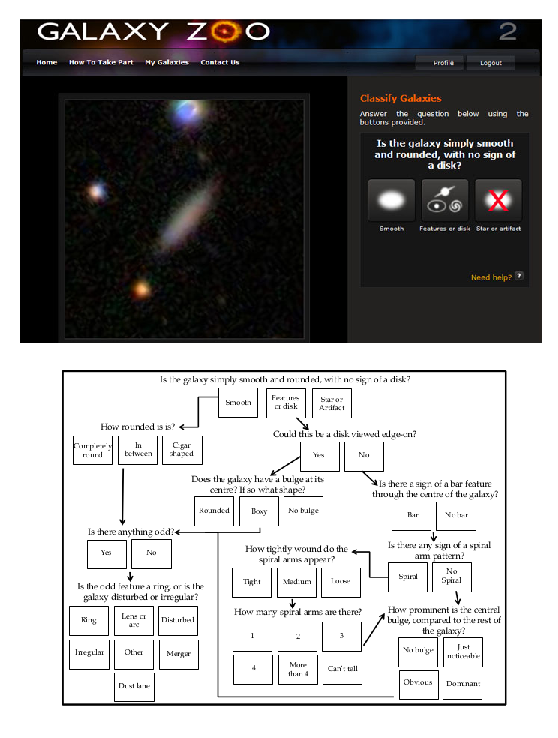
\includegraphics[angle=0,width=3.0in]{figures/interface.eps}
\caption{{\it Top:} Front page of the web interface for Galaxy~Zoo~2, displaying Task~01. {\it Bottom:} Flowchart of the 11 classification tasks for GZ2, beginning at the top centre. 
\label{fig-interface}}
\end{figure}

The Galaxy~Zoo~2 tree has 11 classification tasks with a total of 37 possible responses (Table~\ref{tbl-tree}). A classifier selects only one option for each task, after which they are immediately taken to the next step in the tree. Task~01 is the only question answered for all objects in the sample. Once a classification was completed, an image of the next galaxy is automatically displayed and the user can begin on a new object. 

\begin{table}
 \caption{GZ2 classification tree \label{tbl-tree}}
 \begin{tabular}{@{}cllr}
 \hline
\multicolumn{1}{l}{Task} &
\multicolumn{1}{c}{Question} &
\multicolumn{1}{c}{Responses} &
\multicolumn{1}{c}{Next} 
\\ 
\hline
\hline						% Mean N_class for Task 01
01    & {\it Is the galaxy simply smooth   }  & smooth           & $\rightarrow$~07 \\
      & {\it and rounded, with no sign of  }  & features or disk & $\rightarrow$~02 \\
      & {\it a disk?                       }  & star or artifact & {\bf end} \\
      \hline
02    & {\it Could this be a disk viewed   }  & yes              & $\rightarrow$~09 \\
      & {\it edge-on?                      }  & no               & $\rightarrow$~03 \\
      \hline
03    & {\it Is there a sign of a bar      }  & yes              & $\rightarrow$~04 \\
      & {\it feature through the centre    }  & no               & $\rightarrow$~04 \\
      & {\it of the galaxy?                }                                        \\
      \hline
04    & {\it Is there any sign of a        }  & yes              & $\rightarrow$~10 \\
      & {\it spiral arm pattern?           }  & no               & $\rightarrow$~05 \\
      \hline
05    & {\it How prominent is the          }  & no bulge         & $\rightarrow$~06 \\
      & {\it central bulge, compared       }  & just noticeable  & $\rightarrow$~06 \\
      & {\it with the rest of the galaxy?  }  & obvious          & $\rightarrow$~06 \\
      & {\it                               }  & dominant         & $\rightarrow$~06 \\
      \hline
06    & {\it Is there anything odd?        }  & yes              & $\rightarrow$~08 \\ 
      & {\it                               }  & no               & {\bf end}        \\
      \hline
07    & {\it How rounded is it?            }  & completely round & $\rightarrow$~06 \\
      & {\it                               }  & in between       & $\rightarrow$~06 \\
      & {\it                               }  & cigar-shaped     & $\rightarrow$~06 \\
      \hline
08    & {\it Is the odd feature a ring,    }  & ring             & {\bf end}        \\
      & {\it or is the galaxy disturbed    }  & lens or arc      & {\bf end}        \\
      & {\it or irregular?                 }  & disturbed        & {\bf end}        \\
      & {\it                               }  & irregular        & {\bf end}        \\  
      & {\it                               }  & other            & {\bf end}        \\  
      & {\it                               }  & merger           & {\bf end}        \\  
      & {\it                               }  & dust lane        & {\bf end}        \\  
      \hline
09    & {\it Does the galaxy have a        }  & rounded          & $\rightarrow$~06 \\
      & {\it bulge at its centre? If       }  & boxy             & $\rightarrow$~06 \\
      & {\it so, what shape?               }  & no bulge         & $\rightarrow$~06 \\
      \hline
10    & {\it How tightly wound do the      }  & tight            & $\rightarrow$~11 \\
      & {\it spiral arms appear?           }  & medium           & $\rightarrow$~11 \\
      & {\it                               }  & loose            & $\rightarrow$~11 \\    
      \hline
11    & {\it How many spiral arms          }  & 1                & $\rightarrow$~05 \\
      & {\it  are there?                   }  & 2                & $\rightarrow$~05 \\
      & {\it                               }  & 3                & $\rightarrow$~05 \\
      & {\it                               }  & 4                & $\rightarrow$~05 \\
      & {\it                               }  & more than four   & $\rightarrow$~05 \\
      & {\it                               }  & can't tell       & $\rightarrow$~05 \\
\hline
 \end{tabular}
 %\medskip
 %\begin{flushleft}
 % Table notes go here.
 %\end{flushleft}
\end{table}

Data from the classifications was stored in a live Structured Query Language (SQL) database. In addition to the morphology classifications, we also registered the timestamp, user identification, and galaxy identification for each asset in the database. 

Galaxy~Zoo~2 was launched on 2009-02-16 with the ``original'' sample of 245,609 images. The ``extra'' galaxies from the Legacy survey were added on 2009-09-02. The normal-depth and first coadded Stripe~82 images were mostly added on 2009-09-02, with an additional $\sim7700$ of the coadded images added on 2010-09-24. Finally, the second version of the coadded images were added to the site on 2009-11-04. 

For most of the duration of Galaxy~Zoo~2, all images were shown to classifiers in a random order. However, we desired to have all galaxies classified a minimum number of times. Therefore, in the final period of Galaxy~Zoo~2, accompanied by a competition with a running tally (dubbed the Zoonometer), objects with low numbers of classifications were shown to users at a higher rate. The goal was a minimum of 40 classifications for the ``original'', ``extra'' and ``stripe82'' samples, and 20 for the ``stripe82\_coadd\_2'' sample. The ``stripe82\_coadd\_1'' sample was removed from the site at this time. The main sample galaxies finished with a median of 44 classifications, with 27\% having fewer than 40; the ``stripe82\_coadd\_2'' galaxies had a median of 21 classifications and 26\% of them had fewer than 20 (Table~\ref{tbl-sample}). 

The last GZ2 classifications were collected on 2010-04-29, spanning a period of just over 14 months. The final dataset contained 16,340,298 classifications (comprising a total of 58,719,719 questions) by 83,943 participants.

\begin{comment}
\subsection{Comparing the main and additional samples}\label{ssec-mainsample}

\begin{figure*}
\includegraphics[angle=0,width=7.0in]{figures/check_children.eps}
\caption{{\it Top:} comparison of the galaxy properties for the ``original'' (red), ``extra'' (blue), and a matched subsample of the ``original'' (green). Histograms show the distributions of the galaxies based on $(u-r)$ colour (left), Petrosian $m_r$ (centre), and the Petrosian $r$-band 50\% angular radius (right). The thick lines show the normalized sample distributions, while the thin lines correspond to their cumulative probability distributions. {\it Bottom:} Distribution of selected GZ2 weighted vote fractions (minimum 20 votes per task) for only the ``extra'' and sub-selected ``original'' samples. The distributions are consistent for Tasks 01 (left) and 03 (right); Task 02 (middle) shows a moderate decrease in strong ``no'' vote fractions for edge-on disks for the ``extra'' sample.
\label{fig-original_vs_extra}}
\end{figure*}

It is important to check that a significant difference does not exist between the original sample and those galaxies in the extra sample that were added later. The median distribution of classifications for the ``extra'' sample is only slightly lower than that of the ``original'' sample (41 compared to 44), although slightly bimodal. Since the ``extra'' sample was introduced at a later time, however, we tested for potential classification biases that could occur with a different base of users. 

The galaxies included in the ``extra'' sample have a slight tendency to be brighter in $r$-band than the ``original'' sample, and are on average both larger and bluer (Figure~\ref{fig-original_vs_extra}). This is a result of the deblending issues that led to their selection -- since the galaxies themselves are identified as blended, they have a larger area and multiple brightness peaks. Such peaks are commonly caused by distinct regions of star formation within a galaxy, leading to their bluer colours. 

We constructed a sub-sample of $\sim16,000$ ``original'' galaxies that match the brightness, colour, and angular size distribution of the ``extra'' sample. Comparing the GZ2 vote fractions of these galaxies to the ``extra'' sample shows excellent agreement for almost all tasks, with a difference in the mean vote fractions of less than 5\% (Figure~\ref{fig-original_vs_extra}). A series of binned Kolmogorov-Smirnov tests show that there are only two tasks for which the distributions are inconsistent above the $2\sigma$ level. The first includes several responses to Task 08 (odd feature), in which vote fractions are subject to large variances due to the rarity of the phenomena (dust lanes, arcs, etc.) and the larger number of possible responses. Since the votes for all these responses are dominated at the low end, we do not consider this strong evidence for any bias. The second is Task 02 (edge-on; $p_{KS}<0.08$), for which the ``extra'' sample showed a slightly higher rate of identifying edge-on disks than in ``original'' galaxies. This could be evidence that classifiers became more adept over time at distinguishing disks from highly elliptical early-type galaxies; there is in addition a smaller difference in the vote fractions for ``cigar-shaped bulge'', for which it could conceivably be confused.  

Given the small differences across almost all classifications for the two samples, we elect to use the union of the ``original'' and ``extra'' galaxies as the GZ2 main sample. All reduction and analysis in the remainder of this paper will apply to this combined sample; however, the catalogue maintains a separate column that distinguishes between them and can be used by researchers concerned with further time-dependent biases. 

The magnitude-limited ''stripe82\_normal'' data showed even better agreement of its GZ2 raw vote distributions when compared to the ``original'' sample ($p_{KS}>0.1$ for all tasks). These galaxies can also be added as the third component of the ``main'' sample -- the debiasing should be run separately on this combined set to see what the results are.  

\subsection{Stripe~82 samples}\label{ssec-s82samples}

The ``stripe82'' normal-depth sample was selected in exactly the same manner as the standard sample, aside from the removal of the {\tt In Legacy} flag, the addition of ra and dec restrictions to select the appropriate region of sky, and a fainter limit of petroMag\_r (Galactic-extinction corrected) $< 17.77$. This resulted in 21,522 objects.

The ``stripe82\_coadd'' sample is constructed from the union of two selections. The first selection proceeds in the same manner as the standard sample, but using the stripe82 database, rather than DR7, limited to the coadd runs 106 and 206, and to petroMag\_r (Galactic-extinction corrected) $< 17.77$. Due to differences in deblending and photometry between the normal- and coadd-depth imaging, there were a significant number of objects in the normal-depth catalogue which were not in the coadd-depth catalogue. A second selection therefore matched objects in the normal-depth ``stripe82'' sample to the full coadd table. The matching algorithm finds all coadd objects within 1~petroR90\_r of an object in the normal-depth catalogue and selects the object with the lowest figure-of-merit, defined as $(dr + 0.01\times dm)$, where $dr$ is the positional difference in arcmin and $dm$ is the magnitude difference in mag (i.e., 1~mag is equivalent to 0.6~arcsec).

The ``stripe82\_coadd'' sample selection resulted in 30,400 objects, a few dozen of which did not appear in GZ2 due to problems creating the colour images (mostly related to mosaicing). The final ``stripe82\_coadd\_1'' sample contains 30,346 objects and the ``stripe82\_coadd\_2'' sample contains 30,339 objects. The '``stripe82\_coadd\_1'' and ``stripe82\_coadd\_2'' samples are nearly identical in the objects comprising them; only the method used to create the images is different.

The construction of the ``stripe82\_coadd'' sample was designed to enable maximum overlap with a sample selected from the normal-depth catalogue. To obtain a homogeneously-selected sample from the coadd-depth imaging alone one must reapply the magnitude and size cuts to the ``stripe82\_coadd'' sample.

A final complication is that the SDSS stripe82 database does not provide matches to spectra; these were determined by finding the best redshift measurement (if any) within $1.2\arcsec$ of the coadd object's position.

\end{comment}

%%%%%%%%%%%%%%%%%%%%%%%%%%%%%%%%%%%%%%%
%%%%%%%%    Data reduction       %%%%%%%%%%%%%
%%%%%%%%%%%%%%%%%%%%%%%%%%%%%%%%%%%%%%%

\section{Data reduction} \label{sec-datareduction}

\subsection{Multiple classifications}
In a small percentage of cases, an individual user may classify the same object more than once. Since we wish to treat each click as an independent measurement, we removed multiple classifications of the same object by a given user from the data, keeping only the last submitted classification. Such repeats only occurred for a small proportion of objects ($\sim1\%$), with only a tiny proportion ($\sim0.01\%$) occurring enough to significantly alter the final vote fractions. 

\subsection{Consistency and invididual user weighting}\label{ssec-consistency}

The next step in reducing the data is to remove the influence of unreliable users. To do so we applied an iterative weighting scheme. First, we calculated the vote fraction ($f_r = n_{r}/n_{task}$) for every answer for every task for every object, weighting each user's vote equally. Here, $n_r$ is the number of clicks for a given answer and $n_{task}$ is the total number of clicks for that task. Individual clicks are then compared to the vote fraction to calculate its consistency $\kappa$:

\begin{equation}
\kappa = \frac{1}{N_r}\sum_i{\kappa_i},
\label{eqn-consistency}
\end{equation}

where $N_r$ is the total number of possible reponses for a task and: 
\begin{equation}
    \kappa_i = \left\{
    \begin{array}{l l}
      f_r       & \text{ if click corresponds to this answer,} \\
      (1 - f_r) & \text{ if click does not correspond.}\\
    \end{array} \right.
    \label{eqn-consistency2}
 \end{equation}

For example, if a question has three possible answers, and the galaxy corresponds best to answer $a$, then the vote fractions for answers $(a, b, c)$ might be $(0.7, 0.2, 0.1)$.
\begin{itemize}
\item If an individual selected answer $a$, then $\kappa = (0.7 + (1-0.2) + (1-0.1))/3 = 0.8$
\item If an individual selected answer $b$, then $\kappa = ((1-0.7) + 0.2 + (1-0.1))/3 = 0.467$
\item If an individual selected answer $c$, then $\kappa = ((1-0.7) + (1-0.2) + 0.1)/3 = 0.4$
\end{itemize}
\noindent Clicks which agree with the majority thus have high values of consistency, whereas clicks which disagree have low values.

\begin{figure}
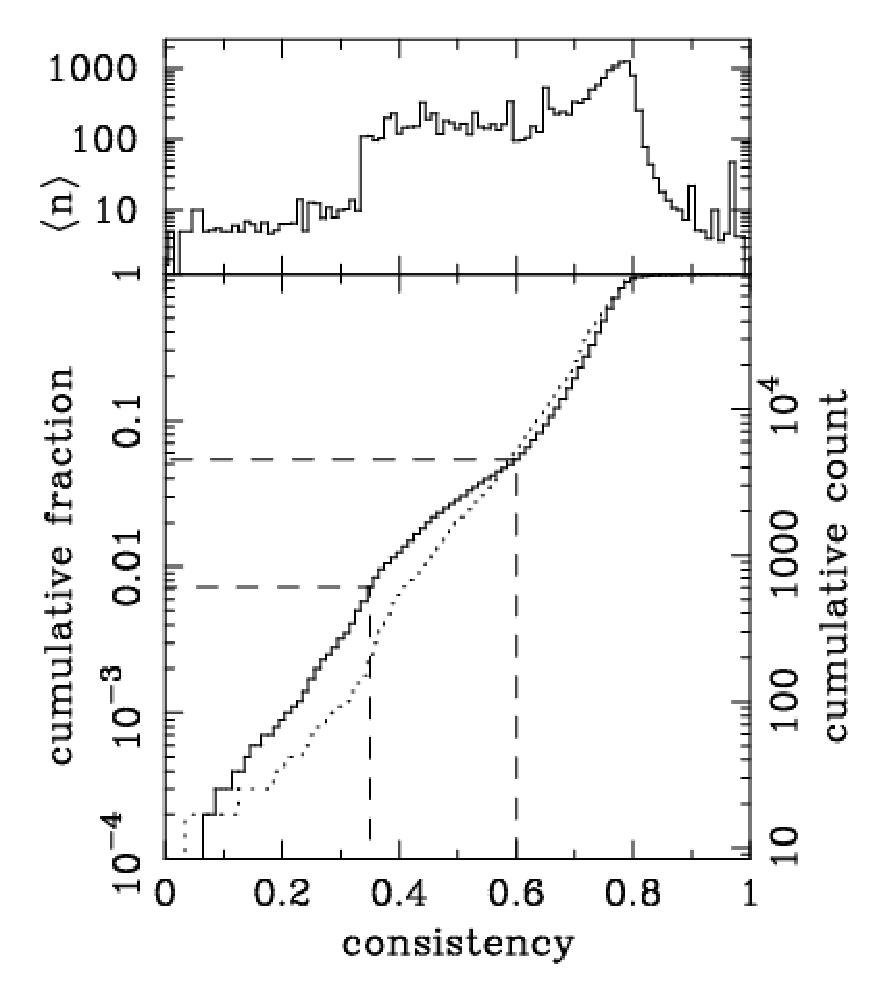
\includegraphics[angle=0,width=3.3in]{figures/user_consistency.eps}
\caption{User consistency for Task XX. Top: total number of galaxies classified per user as a function of their consistency. Bottom: Cumulative fraction distribution of consistency. The dotted line shows the first iteration of weighting, and the solid line the third iteration. The second iteration is not shown, but is almost identical to the third. 
\label{fig-consistency}}
\end{figure}

Based on the distribution of results for the initial iteration of $\kappa$ (Figure~\ref{fig-consistency}), we chose a weighting function that down-weighted users in the tail of low consistency:

\begin{equation}
w = \text{power}((\kappa/0.6),8.5)
\label{eqn-weight}
\end{equation}

\noindent For this function, $w=1$ for $\sim95\%$ of users and $w<0.01$ for only $\sim1\%$ of users. The vast majority of users are thus treated equally: there is no up-weighting of the most consistent users. The top panel of Figure~\ref{fig-consistency} also shows the lowest-weighted users have on average classified only a handful of objects.

After computing $\kappa$ for all tasks, the vote fractions were recalculated using the new user weights. We repeated this process a third time to ensure convergence. For each task, this produces both a weighted number of votes and a weighted vote fraction for each task. 

\subsection{Classification bias}\label{ssec-classificationbias}

The weighted vote fractions in the data are also adjusted for what we term {\it classification bias}. The overall effect is a change in observed morphology fractions as a function of redshift, a trend seen in the original Galaxy~Zoo~1 data. The presumed cause is that more distant galaxies are, on average, both smaller and dimmer as they appear in the cutout images; as a result, finer morphological features are more difficult to identify. 

Figure~\ref{fig-type_fractions} demonstrates the classification bias for several of the Galaxy~Zoo~2 classification tasks. The average weighted vote fraction for each response ({\it thin lines}) is shown as a function of redshift; the fraction of votes for finer morphological features (such as identification of disk galaxies, spiral structure, or galactic bars) decrease at higher redshift. The trend is strongest for the initial classification of smooth and feature/disk galaxies, but almost all tasks exhibit some level of change. Part of this effect is due to the nature of a luminosity-limited sample; high-redshift galaxies must be more luminous to be detected in the SDSS and are thus more likely to be giant red ellipticals. However, we see evidence of the classification bias even in magnitude-limited samples. Since this bias contaminates any potential studies of galaxy demographics over the entire volume of the sample, it must be corrected to the fullest possible extent. 

\begin{figure*}
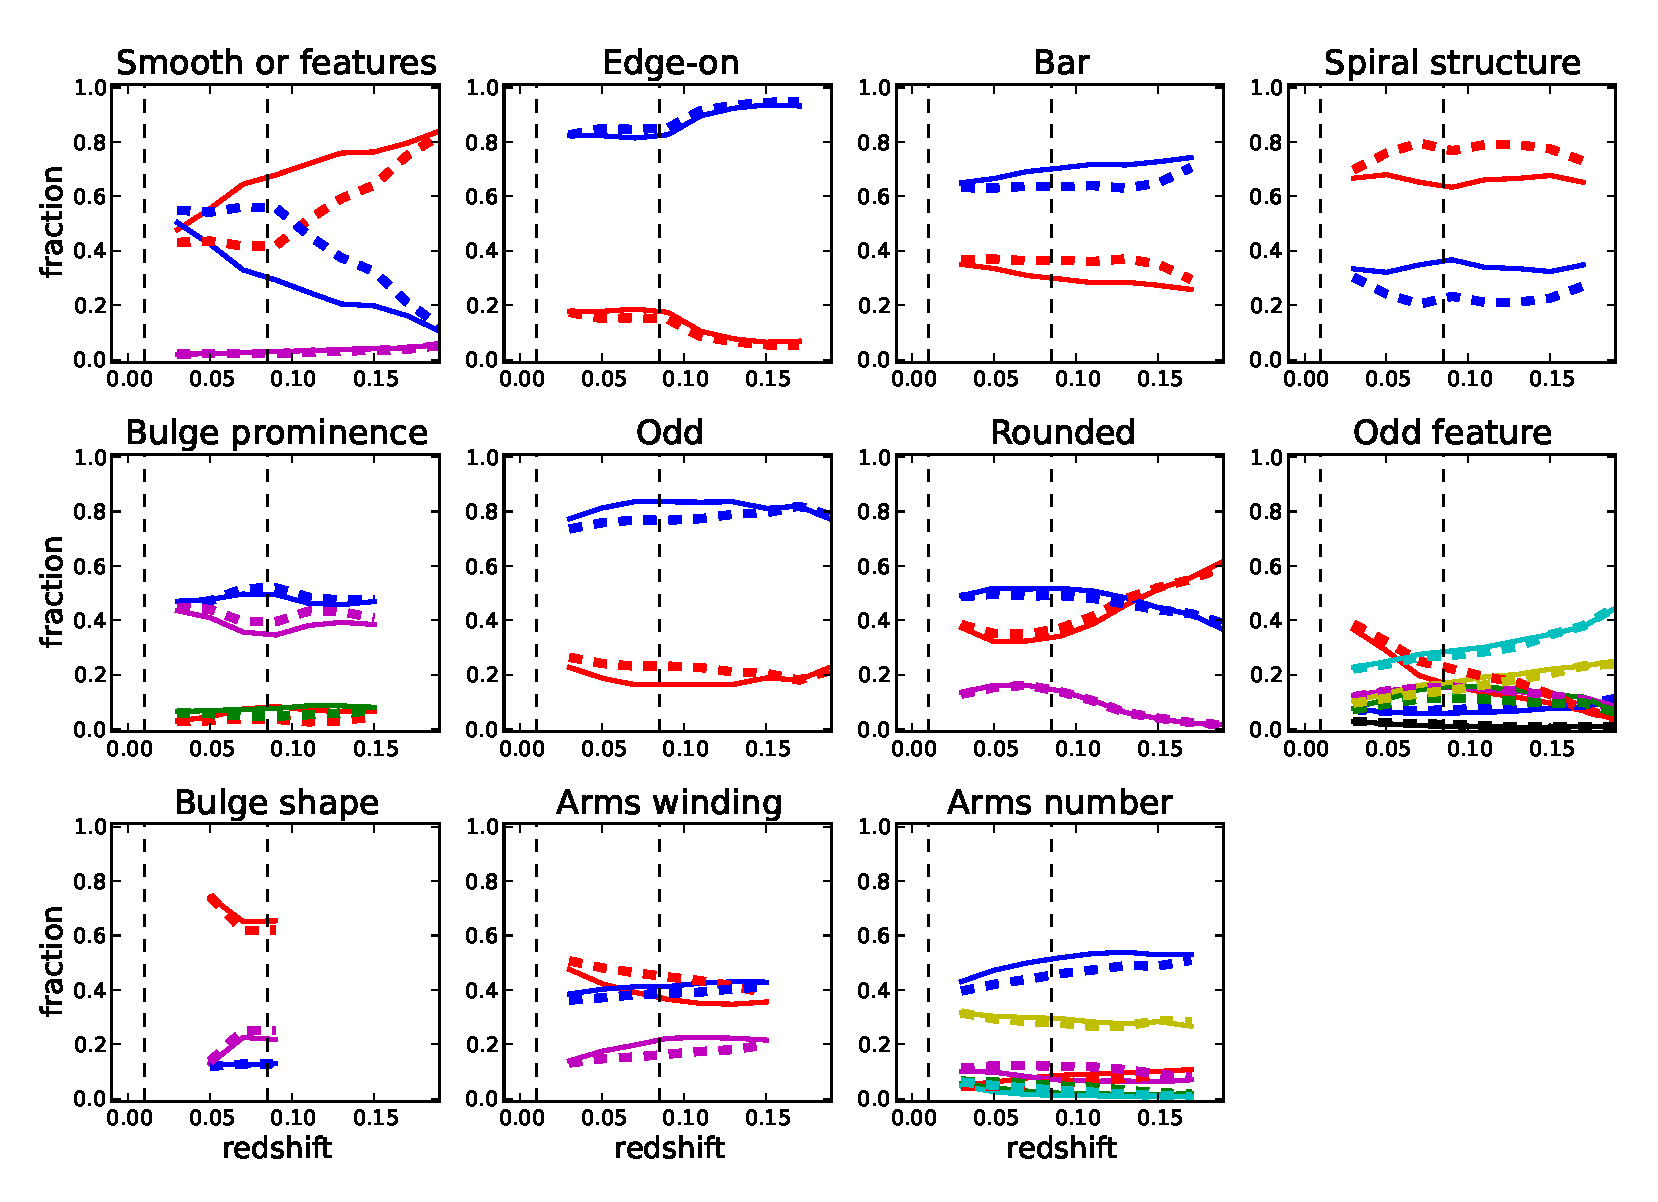
\includegraphics[angle=0,width=7.0in]{figures/gz2_type_fractions.eps}
\caption{Type fractions for the classification tasks in GZ2. Solid (thin) lines show the weighted vote fractions, while the thick (dashed) lines show the debiased vote fractions that have been adjusted for classification bias. This is a magnitude-limited sample for \mr~$<-20.17$. Vertical dashed lines show the redshift at $z=0.01$ (the lower limit of the correction) and $z=0.085$ (the redshift at which the absolute magnitude limit reaches the sensitivity of the SDSS). 
\label{fig-type_fractions}}
\end{figure*}

\citet{bam09} corrected for classification bias in the original Galaxy~Zoo data, but only for the elliptical and combined spiral variables. Their approach was to bin the galaxies a function of absolute magnitude (\mr),the physical Petrosian half-light radius (\rfifty), and redshift. They then measure the average elliptical-to-spiral ratio for each (\mr,\rfifty) bin in the lowest available redshift slice; this yields a local baseline relation which gives the (presumably) unbiased morphology as a function of the galaxies' {\em physical}, rather than {\em observed} parameters. From the local relation, they derive a correction for each (\mr,\rfifty,$z$) bin and then adjust the vote fractions for the individual galaxies in each bin. The validity of this approach is justified in part by the agreement of these debiased probabilities with a monotonic morphology-density relation \citep{bam09}. We modify and extend this technique for the Galaxy~Zoo~2 classifications. 

There are two major differences between the GZ1 and GZ2 data. First, GZ2 has a decision tree, rather than a single question and answer for each click on an image. This means that all tasks, with the exception of the first, depend on answers to previous classifications in the tree. For example, the bar question is only asked if the user classifies a galaxy as having ``features or disk'' and as ``not edge-on''. Thus, the value of the weighted vote fraction for this example task only addresses the total bar fraction {\em among face-on disk galaxies}, and not as a function of the general population. 

Our approach is to examine only biases within the context of the individual classification tasks. The corrections used to debias each task are derived based only galaxies with sufficient votes to characterize that feature. We emply a combination of threshold on the weighted vote fraction for preceding tasks as well as a lower limit on the total number of votes for a galaxy to be used in deriving a correction. While this increases the number of noisy bins, it is critical for reproducing accurate baseline measurements of individual morphologies. The adjustment derived from well-classified galaxies is then applied to the vote fractions for {\em all} galaxies in the sample. 

The second major issue is the adjustment of the GZ1 vote fractions assumed that the single task was essentially binary. Since almost every vote in GZ1 was either for ``elliptical'' or ``spiral'' (either anticlockwise or clockwise), they were able to use that ratio as the sole metric of the morphology. No systematic debiasing was done for the other GZ1 response options (``star/don't know'', ``merger'', or ``edge on/unclear''), and the method of adjusting the vote fractions assumes that these do not significantly affect the classification bias for the most popular responses. 

Vote fractions for each galaxy are adjusted for classification bias using the following method. The method relies on the assumption that for a galaxy of a given physical brightness and size, a sample of other galaxies with similar brightnesses and sizes will (statistically) share the same average morphologies for a given task. We represent this as the ratio of vote fractions $(f_i/f_j)$ for responses $i$ and $j$. Finally, we assume that the true (that is, unbiased) ratio of likelihoods for each task $(p_i/p_j)$ is related to the measured ratio via a single multiplicative constant:

\begin{equation}
\frac{p_i}{p_j} = \frac{f_i}{f_j}\times K_{j,i}.
\label{eqn-kdef}
\end{equation}

\noindent In this case, the adjusted likelihood for a single task is written as:

\begin{equation}
p_i = \frac{1}{1/p_i},
\label{eqn-adjprob1}
\end{equation}

\noindent and the sum of all the likelihoods for a given task must be unity:
\begin{equation}
p_i + p_j + p_k + \dots = 1.
\label{eqn-sumprob}
\end{equation}

\noindent Multiplying (\ref{eqn-adjprob1}) by (\ref{eqn-sumprob}) yields:

\begin{eqnarray}
p_i &=& \frac{1}{1/p_i} \times \frac{1}{p_i + p_j + p_k + \dots} \\
p_i &=& \frac{1}{p_i/p_i + p_j/p_i + p_k/p_i + \dots} \\
p_i &=& \frac{1}{\sum\limits_{j\ne i}{(p_j/p_i)} + 1} \\
p_i &=& \frac{1}{\sum\limits_{j\ne i}{K_{j,i} (f_j/f_i)} + 1}.
\end{eqnarray}

The corrections for each pair of tasks can be directly determined from the data. At the lowest sampled redshift bin ($z\simeq0$), $\frac{p_i}{p_j} = \frac{f_i}{f_j}$ and $K_{j,i}=1$. From Equation~\ref{eqn-kdef}:

\begin{eqnarray}
\left(\frac{f_i}{f_j}\right)_{z=0} &=& \left(\frac{f_i}{f_j}\right)_{z=z^\prime}\times K_{j,i} \\
K_{j,i} &=& \left(\frac{f_i}{f_j}\right)_{z=z^\prime} / \left(\frac{f_i}{f_j}\right)_{z=0} \\
\end{eqnarray}

\noindent This can be simplified if we define $C_{j,i}\equiv\text{log}_{10}(K_{j,i})$:

\begin{eqnarray}
C_{j,i} &=& \text{log}~\left[\left(\frac{f_i}{f_j}\right)_{z=z^\prime} / \left(\frac{f_i}{f_j}\right)_{z=0}\right] \\
C_{j,i} &=& \text{log}~\left(\frac{f_i}{f_j}\right)_{z=z^\prime} - \text{log}~\left(\frac{f_i}{f_j}\right)_{z=0}.
\end{eqnarray}

\noindent So the correction $C_{j,i}$ for any bin is simply the difference between $f_i/f_j$ at the desired redshift and between that of a local baseline, where the ratios between vote fractions are expressed as logarithms.  

The local baselines and subsequent corrections are derived from the main sample data (original + extra + magnitude-limited Stripe~82). Since determining the baseline ratio relies on absolute magnitude and physical size, we only use the 86\% of galaxies in the main sample with spectroscopic redshifts. We also use only galaxies with sufficient numbers of classifications to determine the morphology ratios. This varies as a function of the task -- for the questions asked of every galaxy (Tasks 01 and 06), we set the minimum number of classifications at 30. This is well below the median of 43, and includes $>97\%$ of the sample. For other tasks with fewer total responses, this can be as low as 10 classifications per task. 

The weighted vote fractions for each task response are binned in three dimensions: the absolute magnitude \mr, the Petrosian $r$-band half-light radius \rfifty, and redshift $z$. Bins range for \mr~range from $-24$ to $-16$ in steps of 0.25~mag, for \rfifty~from 0 to 15~kpc in steps of 0.5~kpc, and for $z$ from $0.01$ to $0.26$ in steps of 0.01. The bin ranges and step sizes are chosen to maximize the phase space covered by the bias correction, while also retaining enough galaxies in each bin to establish its morphology distribution. The value of each bin in the cube is the sum of the weighted vote fractions for that response. For each pair of responses $(i,j)$ to a question, we compute log$(f_j/f_i)$ in every (\mr,\rfifty,\redshift) bin. The local baseline relation is established by selecting the value in the non-empty bin(s) for the lowest-redshift slice at a given (\mr,\rfifty). 

Since each unique pair of responses to a question will have a different local baseline, there are $\binom{n}{2}$ corrections for a task with $n$ responses. This reduces to the method with a single pair of variables described in \citet{bam09} if $n=2$. 

\begin{figure*}
\includegraphics[angle=0,width=7.0in]{figures/gz2_baselines.eps}
\caption{Local morphology ratios for morphology classifications in GZ2. The ratio of the binned vote fractions for morphologies is for the first two responses in the decision tree (Table~\ref{tbl-tree}) for each task; there may be as many as 21 such pairs for tasks with more than two options. The dashed horizontal lines give the physical scale corresponding to $1\arcsec$, while the curved lines show a constant apparent surface brightness of $\mu_{50,r}=23.0$~mag~arcsec$^{-2}$.
\label{fig-baselines}}
\end{figure*}

The baseline morphology ratios for the GZ2 tasks are shown in Figure~\ref{fig-baselines} for the first two responses in each task. To derive a correction for bins not covered at low redshift, we attempted to fit each baseline ratio with an analytic, smoothly-varying function. The baseline ratio for the ``smooth'' and ``features/disk'' responses to Task 01 is functionally very similar to the GZ1 relation \citep[Figure~A5 in ][]{bam09}, as expected. It is reasonably well-fit with an analytic function of the form:

\begin{equation}
\frac{f_j}{f_i}[R_{50},M_R] = \frac{s_6}{1 + exp[(x_0 - M_R)/x_1]} + s_7
\label{eqn-sb}
\end{equation}

\noindent where:

\begin{eqnarray}
\alpha &=& s_2^{-\left(s_1 + s_8{R_{50}}^{s_9}\right)} + s_3 \\
\beta  &=& s_4 + s_5(x_0 - s_3)
\end{eqnarray}

\noindent and where $\{s_1,s_2,s_3,s_4,s_5,s_6,s_7,s_8,s_9\}$ are minimized to fit the data. The only other task had baseline ratios reasonably well fit by these parameters was Task~07 (rounded smooth galaxies). We adopted the same approach for this task and were able to fit the behavior of all three pairs of responses with the same functional form. 

None of the other tasks are well-fit by a function of the form in Equation~\ref{eqn-sb}; for these, we instead adopt a simpler fit where both \mr~and \rfifty~vary linearly:

\begin{equation}
\frac{f_j}{f_i}[R_{50},M_R] = t_1(R_{50} - t_2) + t_3(M_R - t_4) + t_5,
\label{eqn-tilt}
\end{equation}

\noindent and $\{t_1,t_2,t_3,t_4,t_5\}$ are the parameters to be minimized. We fit Equation~\ref{eqn-tilt} to all other tasks where the number of bins is sufficient to get a reasonable fit. Finally, for pairs of responses with only a few sampled bins, we instead used the direct difference between the local ratio and the measured ratio at higher redshift. Galaxies falling in bins that are not well-sampled are assigned a correction of $C_{i,j}=0$ for that term; this is necessary to avoid overfitting based on only a few noisy bins. 

%The baseline ratio of the edge-on task for disk galaxies (upper right, Figure~\ref{fig-baselines}) is still a reasonably strong function of both \mr~and \rfifty; however, the form of Equation~\ref{eqn-sb} produces a poor fit to the data. The bar and spiral structure questions for face-on disk galaxies (lower panels, Figure~\ref{fig-baselines}) have very different behavior; the bar/no~bar ratio shows no strong dependence on either \mr~or \rfifty, where the spiral/no~spiral ratio resembles that for Task~01. 

%For pairs of responses that have well-behaved ratio estimates, we fit them with an algebraic function in \mr~and \rfifty~and adopt the fit as the baseline. For responses for which no good fit can be determined, we use the values of the bins directly as the baseline. For the few galaxies that lie in bins outside the corrected area, we use the mean correction for the nearest neighbours within 1.2 times the distance to the bin centre {(\bf TO BE IMPLEMENTED)}. 

The success of this method is generally good for most GZ2 tasks and responses. Figure~\ref{fig-type_fractions} illustrates the comparison between the raw and debiased vote fractions. The debiased results ({\it thick lines}) are generally flat over a range of $0.01<z<0.085$, where $L^\star$ galaxies fall below the magnitude limit of the survey and the bins are more poorly sampled. The debiased early- and late-type fractions of 0.45 and 0.55 agree with the GZ1 type fractions derived by \citet{bam09}. The bar fraction in disk galaxies is roughly 0.35, which is slightly higher than the value found by using thresholded GZ2 data in \citet{mas11c}.

\begin{figure*}
\includegraphics[angle=0,width=7.0in]{figures/gz2_bias_demo_task01.ps}
\caption{GZ2 weighted vote fractions for Task 01 ({\it smooth, features/disk, or star/artifact?}) as a function of spectroscopic redshift. The left graph shows the fraction of galaxies for which a category exceeded a threshold of 0.8. Galaxies which had no answer above the threshold are labeled as ``unclassified''. The right shows the mean of the vote fractions, weighted by the total number of responses to the task for each galaxy. Data are shown for the GZ2 original + extra (thick solid), Stripe~82 normal-depth (thin dotted), and Stripe~82 co-add depth (thin solid) samples. Stripe~82 data is only for galaxies with $r < 17.0$, the same magnitude limit applied to the GZ2 main sample.  
\label{fig-task01}}
\end{figure*}

%%%%%%%%%%%%%%%%%%%%%%%%%%%%%%%%%%%%%%%
%%%%%%%%    Catalog       %%%%%%%%%%%%%
%%%%%%%%%%%%%%%%%%%%%%%%%%%%%%%%%%%%%%%

\section{The catalog} \label{sec-catalog}

Other possible inclusions for catalog:
\begin{itemize}
	\item Metrics on classification confidence \citep[Table 04,][]{lin11}
	\item Galaxy Wars
	\item \mr,\rfifty,$z$ bins for each galaxy
	\item Voronoi tessellation bins
	\item Matched SDSS metadata
\end{itemize}

\subsection{Main sample}\label{ssec-catalog_main}

The data release for Galaxy~Zoo~2 consists of four tables, abridged portions of which appear in this paper. Table~\ref{tbl-mainclass} contains classification data for the 283,971 galaxies in the main sample. Each galaxy is identified by its unique SDSS DR7 objID, as well as its original sample designation (either original, extra or Stripe~82 normal-depth). $N_{class}$ is the total number of users who have classfied the galaxy, while $N_{votes}$ gives the total number of clicks summed over all classifications and all responses. For each of the 37 morphological classes, we give six parameters: the raw number of votes for that response (eg, {\tt t01\_smooth\_or\_features\_a01\_smooth\_count}), the number of votes weighted for consistency ({\tt $^\star$\_weight}), the fraction of votes for the task ({\tt $^\star$\_fraction}), the vote fraction weighted for consistency ({\tt $^\star$\_weighted\_fraction}), the debiased likelihood ({\tt $^\star$\_debiased}), which is the weighted fraction adjusted for classification bias (see Section~\ref{ssec-classificationbias}), and a boolean flag ({\tt $^\star$\_flag}) that is set if the galaxy is included in a clean, debiased sample.

Flags for each morphological parameter are determined by applying three criteria: the first is the requirement that more than 50\% of votes for preceding task(s) must eventually select for the task being flagged. For example, to select clean barred galaxies, we require both $p_{features/disk}\geq0.5$ and $p_{not edge-on}\geq0.5$. Secondly, the object must exceed a minimum number of total votes (ranging from 5--30) for that task, in order to eliminate variance from small-number statistics. Finally, we establish a threshold value for the debiased vote fraction; this is 0.5 for Tasks~02 and 03, and 0.8 for all other tasks. GZ1 also used a debiased threshold value of 0.8, based on a correction applied to raw vote fractions at the same threshold \citep{bam09,lin11}. 

Table~\ref{tbl-mainclass_photoz} shows the GZ2 classifications for main sample galaxies without spectroscopic redshifts. To derive the debiased likelihoods, we used the morphology corrections derived from galaxies in the spectroscopic main sample. We then used the photometric redshift provided by the SDSS to derive \mr,\rfifty~and select the appropriate correction bin. The mean redshift error in the photometric sample is $\Delta~z=0.021$ (a fractional uncertainty of 27\%), compared to the spectroscopic accuracy of $\Delta~z=0.00016$ (0.3\%). Since the size of the redshift bins in $C_{j,i}$ is 0.01, a shift of 2--3 bins can potentially produce a very large change in the debiased vote fractions. For this reason, we separate galaxies with spectroscopic and photometric redshifts, and do not recommend that the debiased likelihoods be combined for analysis. 

%Table~\ref{tbl-gz2_s82_remainder} contains the Stripe~82 galaxies with $r>17.0$. 

\subsection{Stripe~82}\label{ssec-s82}

Table~\ref{tbl-stripe82} contains data for the co-added images in Stripe~82. These classifications are for the second method of co-adding exposures, and are limited to the 65\% of the sample with spectroscopic redshifts. Since there are only $\sim10\%$ of the number of galaxies used in the main sample, there are not enough classifications to robustly derive a correction from the data itself. The debiased probabilities for this sample therefore apply corrections based on those in the GZ2 main sample. Flags for these galaxies use the same 50\% criteria as thresholds for previous tasks; however, since galaxies are only classified an average of 21 times each, the number of votes per task is relaxed to 10~votes for Tasks~01 and 06 and 5~votes for all other tasks. 

The distribution of votes for the main sample is similar enough to the Stripe~82 normal-depth (with $r<17.0$) that the same bias correction applies for both. Table~\ref{tbl-stripe82compare} shows the tasks in the GZ2 question tree and the mean weighted vote fraction for each response. The distributions for both the main sample and Stripe~82 galaxies are quite similar, with the difference in the mean varying by $<10\%$ for almost all responses. The only exceptions to these are for responses that target rare objects (and thus are subject to higher variance for low-number statistics), such as dust lanes, rings, and high-multiplicity spiral arms. 

The right panel of Figure~\ref{fig-task01} shows that the weighted vote fractions also behave similarly as a function of redshift, particularly in the $0.01<z<0.08$ range covered by the GZ1 debiasing technique. The agreement is generally good between the Stripe~82 normal depth and the GZ2 main sample; this is not the case for the coadded Stripe~82 data, however. For Task~01, fewer galaxies are classified as robustly smooth (above the 0.8 threshold), moving instead to the ``unclassified'' category. Coadded data showed similar higher fractions of galaxies with bars and for possessing visible spiral structure. A possible cause for this is that the new image pipeline in the coadded data allows viewers to see faint features or disks, due to improved seeing in the coadded data \citep[from $1.4\arcsec$ to $1.1\arcsec$;][]{ann11}.

%What needs to be done:
%\begin{itemize}
%	\item Verify that the normal-depth Stripe~82 vote fractions are similar to the original + extra samples. {\bf Yes.} 
%	\item See whether co-added images follow a different distribution, esp. as function of $z, R_{50}, M_r, \mu$. {\bf They do, even accounting for the magnitude cut.} 
%	\item Decide which of the two co-added samples is more reliable for debiasing efforts. {\bf The only difference between the two samples is a moderate increase in spiral fraction for disk galaxies in coadd1 data. The results of K-S tests on the weighted vote fractions are confusing. Very similar distributions (by eye) have very low probabilities according to the K-S test. Perhaps quote the various moments instead.} 
%%	\item optional: {\it Do a PCA on the normal vs. coadded versions. Figure out which of the four parameters. and in what weighted combination, produces the most scatter in the data. }
%	\item How far out in redshift can we correct the normal data using coadd? Need enough galaxies per bin in $M_r$, $R_{50}$, $z$ space {\em for each task} in the Stripe~82 data to establish the baseline. {\bf 20 galaxies per bin at $\Delta M_r=0.4~\rm{mag}, \Delta R_{50}=0.8~\rm{kpc}, \Delta z = 0.01$ covers a comparable amount of parameter space compared to the GZ1 results of B09.}
%	\item Figure out how the vote fractions are going to be adjusted once a bias has been identified. {\bf Have attempted to correct results for binary tasks based on the B09 method.}
%	\item Apply corrections to the vote fractions in the GZ2 main sample. {\bf Done; works well over redshift range ($0.01<z<0.09$). See Figure~\ref{fig-type_fractions_s82}}.
%\end{itemize}

\begin{figure*}
\includegraphics[angle=-90,width=7.0in]{figures/stripe82_coadd_compare.ps}
\caption{Comparison of GZ classifications from the different coadd techniques for Stripe~82. Left: Distribution of the difference in weighted vote fractions for galaxies that appear in both the coadd1 and coadd2 samples. Each panel shows selected answers in the tree galaxies with at least 10 responses to the task (clockwise from top left: answers 01, 02, 11, and 06). The dashed line shows the median of each distribution; a value of zero means there is no systematic difference, although the widths indicate considerable amounts of scatter for individual classifications. ``Noticeable bulge'' was the only answer in GZ2 for which the mean $|\Delta_{coadd}| > 0.1$. Right: mean values of the difference in the weighted vote fractions for every response in the GZ2 tree. 
\label{fig-stripe82_compare}}
\end{figure*}

%\begin{figure*}
%\includegraphics[angle=0,width=7.0in]{figures/task01_type_fractions.ps}
%\caption{Comparison of GZ Task~01 raw and debiased classifications. Raw classifications are the mean likelihood of all galaxies at each redshift weighted by the number of votes per object. Debiased likelihoods have been adjusted using Equation~\ref{eqn-adjust}. The left panel shows all GZ2 main sample galaxies with redshifts, while the right panel shows all galaxies brighter than $M_r < -20.17$. 
%\label{fig-task01_fractions}}
%\end{figure*}

For almost every response in the GZ2 decision tree, the data (no bias correction) have no systematic differences between classifications using the coadd1 and coadd2 images. Figure~\ref{fig-stripe82_compare} shows distributions of the differences between the two weighted vote fractions ($\Delta_{coadd} = f_{coadd1} - f_{coadd2}$). If the mean value of \dcoadd~for an answer is non-zero, that would indicate a systematic bias in classification due to the image processing. In GZ2, 33/37~tasks have $|\Delta_{coadd}| < 0.05$ (for galaxies with at least 10 responses to the task), with variations in the mean scattered on both sides of \dcoadd. 

The biggest systematic difference is for Task~05, Answer~11 (prominence of the bulge is ``just noticeable''), for which the mean weighted fraction in coadd2 data is $\sim35\%$ higher than from coadd1 data. This is an opposite (but not equal) effect than Answer~12 (obvious bulge), for which the coadd1 data is $\sim13\%$ higher; this may indicate a general shift in votes toward a more prominent bulge. A similar but smaller effect is seen in classification of bulge shapes for edge-on disks (Task~09), where votes for ``no bulge'' in coadd1 data go to ``rounded bulge'' in coadd2. The specific cause for these effects as it relates to the image quality is unknown. 

The comparison of the coadd1 and coadd2 data sets also demonstrates the intrinsic variability in classification of a single object, even with several tens of votes. For example, in the (unbiased) vote fractions from Task~01, 6831 (32.0\%) galaxies from coadd1 and 7,244 (33.9\%) galaxies from coadd2 exceed the ``clean'' early-type threshold of $p\geq0.8$. However, only 2,300 galaxies meet this threshold in {\em both} samples, while the union of the two yields 11,602 galaxies. The difference in numbers between the samples decreases when a higher value of $p$ is used; a more robust jackknife sampling of the data would improve on this 1-sample jackknife. 

%Ellipticals ($p > 0.8$):
%
%coadd 1: 6771
%coadd 2: 7244
%both: 4005
%either: 10219
%
%% Are they close? What is the elliptical percentage of the galaxies that are in coadd1 but not coadd2?
%% Strongly asymmetrical toward cutoff; 62% of the "missing galaxies" have 0.7 < p < 0.8. 
%% Almost identical distribution for ellipticals in coadd2 but not coadd1 (65%)
%
%Spirals:
%
%coadd 1: 1430
%coadd 2: 1826
%both: 1154
%either: 2102

Type fractions for both weighted and debiased vote fractions in normal-depth Stripe~82 are shown in Figure~\ref{fig-type_fractions_s82} for a subset of the GZ2 tasks. The correction flattens the redshift effect in all tasks, similar to the main sample data. The variance along redshift bins is somewhat higher -- formal error bars will need to be computed to see if there is any statistical difference, or whether the result is consistent with a smaller total sample of galaxies.  

\begin{figure*}
\includegraphics[angle=0,width=7.0in]{figures/gz2_stripe82_type_fractions.eps}
\caption{Type fractions for five binary GZ2 tasks for the normal-depth Stripe~82 data. This is a magnitude-limited sample for \mr~$<-20.17$. Vertical dashed lines show the redshift at $z=0.01$ (the lower limit of the correction) and $z=0.085$ (the redshift at which the absolute magnitude limit reaches the sensitivity of the survey). 
\label{fig-type_fractions_s82}}
\end{figure*}

\subsection{Additional data}\label{ssec-metadata}

Although not reproduced in this paper, the repository at \url{http://data.galaxyzoo.org} contains pre-matched tables containing SDSS metadata for the spectroscopic galaxies in the GZ2 main sample. This contains some of the most commonly used DR7 parameters including SDSS exposure information, position, photometry, size, and redshift. Rows are matched to the corresponding galaxies in Tables~\ref{tbl-mainclass}--\ref{tbl-stripe82}. These are provided as a resource for members of the community who wish to compare the morphogical data against external parameters. 

%%%%%%%%%%%%%%%%%%%%%%%%%%%%%%%%%%%%%%%
%%%%%%%%    Comparison       %%%%%%%%%%%%%
%%%%%%%%%%%%%%%%%%%%%%%%%%%%%%%%%%%%%%%

\section{Comparison of GZ2 to other classification methods}\label{sec-comparison}

\begin{itemize}
	\item Galaxy~Zoo~1 \citep{lin11}
	\item \citet{nai10}
	\item \citet{hue11}
%	\item CAS studies \citep{con03,con06} 
	\item EFIGI \citep{bai11}
\end{itemize}

%The main purpose of this section is to perform preliminary comparisons between the weighted, but not debiased data from GZ2 available in early 2012. This analysis will need to be repeated to account for biases in the data; hopefully with the groundwork laid here, it will be faster to repeat it later.  

\subsection{Galaxy~Zoo~1 vs. Galaxy~Zoo~2}

As a check of the classification accuracy, we compare the results from GZ2 to those in GZ1 \citep{lin11}. The galaxies in GZ2 are a subset of those in GZ1, with 248,883 matches between the samples. Task~01 in GZ2 is almost identical to the interface of GZ1. GZ1 allowed for selection of ``merger'' and ``don't know'' options in addition to the first three; and asks for galaxies with ``features or disk'' rather than only for spiral structure. 

The matched GZ1-GZ2 catalog contains 34,480 galaxies flagged as ``clean'' ellipticals based on their debiased GZ1 likelihoods. Of those, 89.0\% had GZ2 raw vote fractions greater than 0.8 and 99.9\% greater than 0.5. Using the GZ2 debiased likelihoods, the vote fractions match at 50.4\% at a threshold of 0.8 and 97.6\% at a threshold of 0.5. 

There are 83,956 galaxies identified as ``clean'' spirals in GZ1. The agreement with the ``features or disk'' response in GZ2, however, is significantly lower. Only 31.6\% of the GZ1 clean spirals had GZ2 raw vote fractions greater than 0.8, with 59.2\% greater than 0.5. The GZ2 debiased likelihoods for the same galaxies only match at 38.1\% (for 0.8) and 78.2\% (for 0.5). 

\begin{figure}
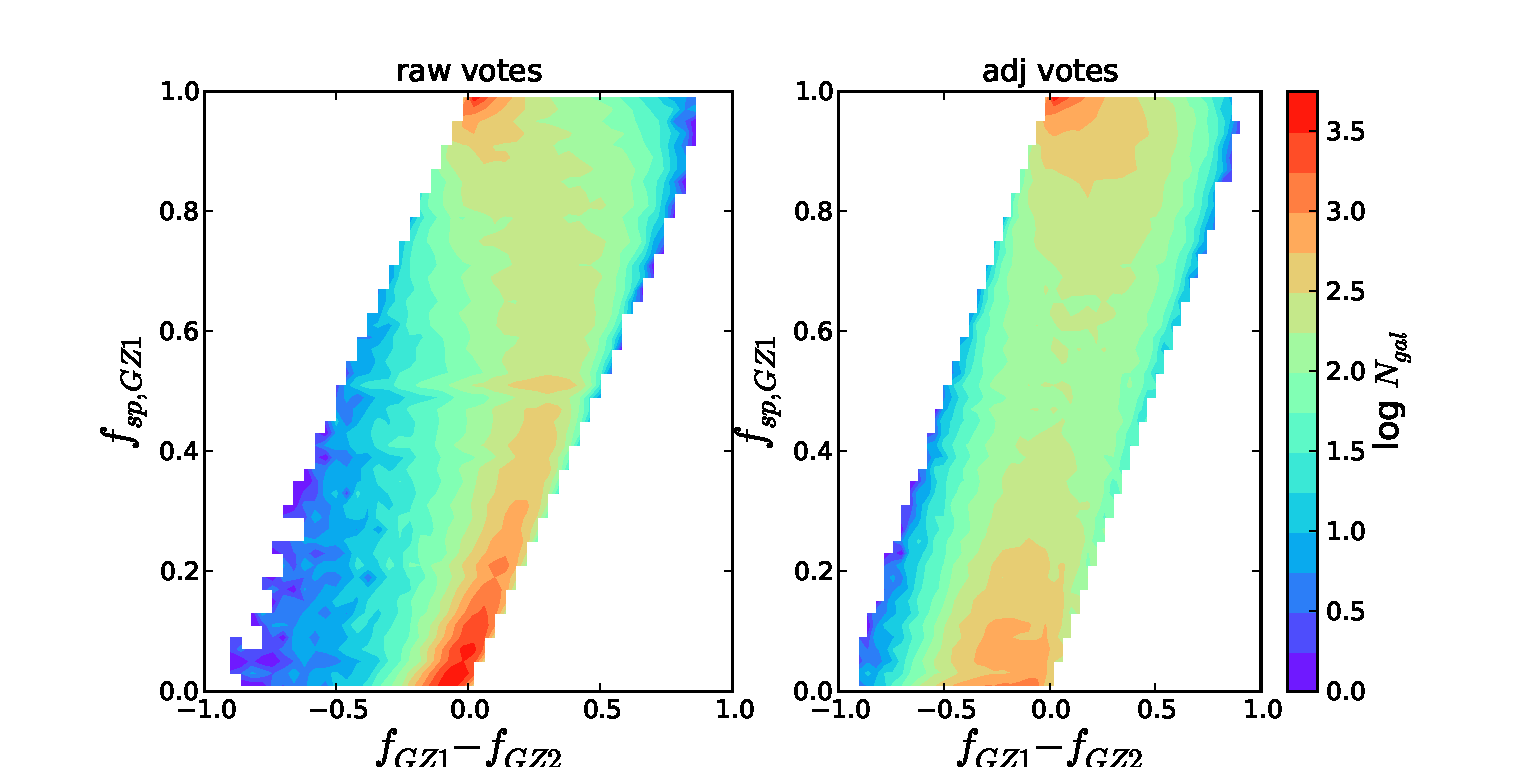
\includegraphics[angle=0,width=3.3in]{figures/gz1_gz2_trumpet.eps}
\caption{Differences in the vote fractions for galaxies in both the Galaxy~Zoo~1 (GZ1) and Galaxy~Zoo~2 (GZ2) projects. Left: Distribution of the differences in the raw weighted vote fractions. Dashed lines show data for all galaxies, while solid lines are for the subset in which $f_{el}$ or $f_{sp} > 0.8$ in both samples. Right: same plot, but using the debiased vote fractions for both samples. 
\label{fig-trumpet}}
\end{figure}

Figure~\ref{fig-trumpet} shows the difference between the vote fractions for the spiral classifications in GZ1 and features/disk classifications in GZ2 for all galaxies that appear in both catalogs. The weighted vote fractions show a tight correlation at both very low and very high values of $f_{sp}$, indicating that both projects agree on the strongest spirals (and corresponding ellipticals). At intermediate ($0.2--0.8$) values of $f_{sp}$, however, GZ1 has vote fractions that are consistently higher than those in GZ2, differing by up to 0.25. When using debiased likelihoods in place of the vote fractions, this effect decreases dramatically; however, the tightness of the correlation correspondingly drops at low and high $f_{sp}$. 

Based on the vote fractions, GZ2 is significantly more conservative than GZ1 at identifying spiral structure. One possible cause for this is a bias from users who are anticipating subsequent questions about the details of any visible structures. If a user clicks ``features or disk'' in GZ2 then an experienced classifier may wish to avoid answering those questions if they are unsure of the classification. They then would be more likely to click ``smooth'' and move on to the next object. With no follow-up questions in GZ1, this would have been less of a concern for the uncertain classifications. We stress that there is no direct evidence for this hypothesis, but suggest it as one possibility for explaining the discrepancy in otherwise identical classification tasks. 

Since the GZ1 vote fractions were specifically directed to galaxies with spiral arms, we also compared GZ1 to the results of Task~04 in GZ2, which specifically asks for spiral structure in already-identified face-on disk galaxies. The agreement with the GZ1 clean spirals is higher than for Task~01, but still well short of that for smooth/elliptical galaxies. Only 63.6\% of galaxies have Task~04 raw vote fractions greater than 0.5 for the GZ1 clean spirals, with 66.8\% for the debiased vote fractions. 

Results from comparing GZ1 to the spiral structure task in GZ2 indicate the robustness of the GZ2 results. If spiral features are identified in GZ2 (having already selected for disk galaxies), then they are very likely to have been seen in GZ1. Conversely, if GZ1 classifications indicate a possible (but not definitive) spiral, it is less likely to appear in GZ2 Task~04, based on the stricter requirements for inclusion. The scatter in the debiased likelihoods may thus be a fair representation of the uncertainty in individual classifications.

\begin{figure*}
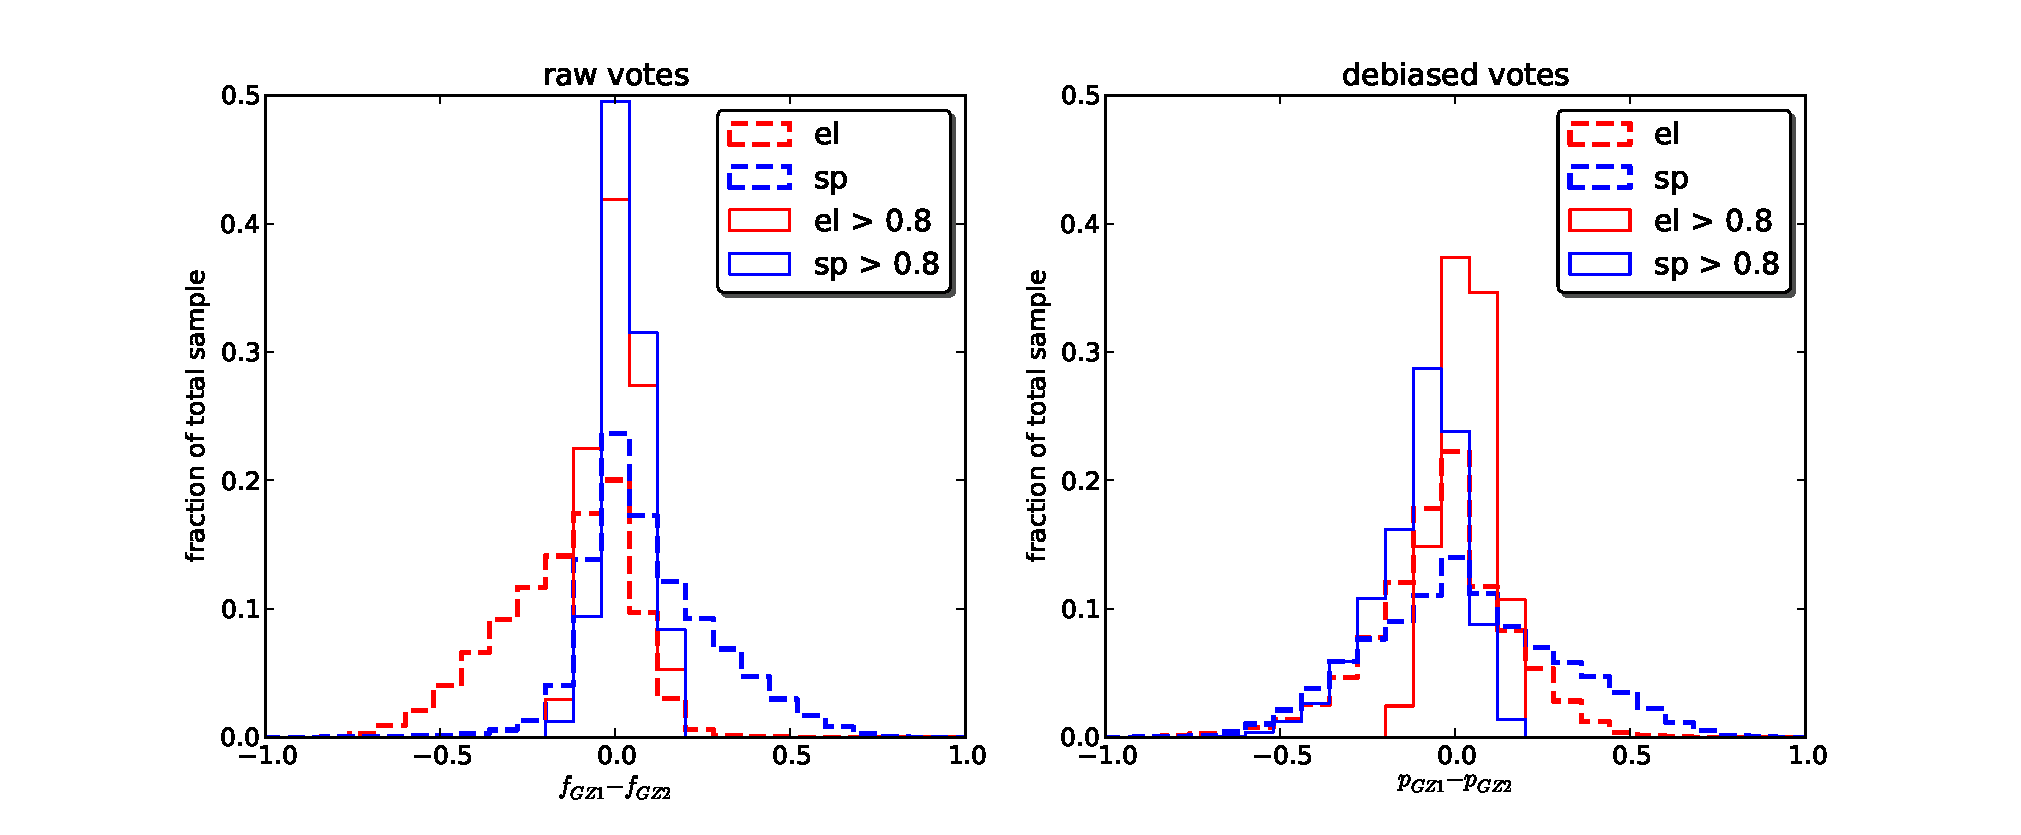
\includegraphics[angle=0,width=7.0in]{figures/gz1_gz2.eps}
\caption{Differences in the vote fractions for galaxies in both the Galaxy~Zoo~1 (GZ1) and Galaxy~Zoo~2 (GZ2) projects. Left: Distribution of the differences in the raw weighted vote fractions. Dashed lines show data for all galaxies, while solid lines are for the subset in which $f_{el}$ or $f_{sp} > 0.8$ in both samples. Right: same plot, but using the debiased vote fractions for both samples. 
\label{fig-gz1_gz2}}
\end{figure*}

Figure~\ref{fig-gz1_gz2} shows the distribution of the difference between the vote fractions for the two projects, using the elliptical and combined spiral data for GZ1 and the Task~01 smooth and ``features or disk'' data for GZ2. For the raw vote fractions, galaxies showed a significant skew toward being more likely to be identified as a spiral in GZ1 than in GZ2. When restricted only to galaxies in the joint CLEAN samples ($p>0.8$), the spread is greatly reduced and the distribution is centred around a difference of zero. The debiased vote fractions show a similar spread when comparing GZ1 and GZ2 classifications, although the skew toward spirals in GZ1 is largely removed. When using only clean galaxies and the debiased vote fractions, galaxies are more likely to be identified as spirals in GZ2. 

The GZ1 interface did have one option that did not classify either early- or late-type galaxies, but rather mergers. This was a rare response in the GZ1 data, comprising less than a percent of the total type fraction at all redshifts \citep{bam09}. \citet{dar10a} found that a weighted vote fraction of $f_{mg} > 0.6$ robustly identified merging systems in GZ1. Of the 1632 systems meeting that criteria and also classified in GZ2, more than 99\% were identified as ``odd'' galaxies, and 77.7\% had a merger fraction above 0.5 as a response to Task~08. This is particularly high when considering that other reponses to that question (such as ``disturbed'', ``irregular'', or ``other'') could conceivably be applied to merging systems. The agreement between GZ1 and GZ2 is surprisingly high, but indicates that mergers were reliably identified in both despite the additional options in the GZ2 question tree. 

\subsection{Nair \& Abraham}

\citet[][hereafter NA10]{nai10} have published a catalog with morphological classifications of 14,034 galaxies from the SDSS DR4. Galaxies were selected from a redshift range of $0.01<z<0.1$, with an extinction-corrected apparent magnitude limit of $g<16$. The overlap with GZ2 is substantial; 12,480 galaxies are found in both catalogs. This comprises nearly all (89.9\%) of the NA10 catalog, but only 4.5\% of GZ2. The GZ2 sample is deeper ($r<17$), spans a wider redshift range ($0.0005<z<0.25$), and contains a more recent data release (DR7) than galaxies in NA10. The large intersection of the two samples makes this an excellent test case to compare morphological classifications from citizen scientists against those done by salaried astronomers.  

\citet{nai10} used classifications by a single professional (P. Nair) to quantify the galactic morphology. She determined RC3 T-types \citep{dev91} for the entire sample through visual inspection of monochrome $g$-band images, covering each source twice. There is no discussion on the procedure if T-types changed between her first and second classifications. 

In addition to the T-types, she also classified various ``fine structure'' morphological features in each galaxy. It is not stated how many times these classifications were performed. These include:

\begin{itemize}
	\item bars (strong, weak, intermediate, ansae, ``peanut'', nuclear, and/or unsure)
	\item rings (nuclear, inner, outer)
	\item lenses [regions of constant surface brightness; not gravitational lenses] (inner, outer)
	\item pairs of objects (close, projected, adjacent, overlapping, + flags for second object type)
	\item interaction (none, disturbed, warp, shells, short tail, medium tail, long tail, bridge)
	\item tails (number)
\end{itemize}

Several of the fine structure features in NA10 can be directly compared to the GZ2 data: namely, bars, rings, and pairs/interactions. All references to the GZ2 vote fraction in the following sections refer to $^\star_weighted_fraction$, which has been weighted but not debiased. 

\subsubsection{Bars}

NA10 detect 2537 barred galaxies, which is 18\% of the total. For objects with T-types later than E/S0, this rises to 25\% of the sample. This is much lower than the fraction found in local galaxies ($\sim60\%$), but similar to the fraction found by \citep{mas11c} for the bar fraction in disky, face-on galaxies from early GZ2 data (29.4\%). 

Two parameters can be set that reduce the number of galaxies in the overlap between the samples, but result in a cleaner cut for comparisons. The first uses the \citet{mas11c} cut for face-on galaxies (log~$(a/b) < 0.3$ using the {\sc expab\_r} parameter from SDSS). The second is to only look at galaxies with at least 10 classifications for task 03 ({\it bar present?}) in GZ2. The reduced face-on sample has 7,121 galaxies from the original 12,480. All trends described below hold generally for both the full overlapping samples and the cleaner face-on sub-sample. Of the objects NA10 identify as barred, 93\% (2348/2537) are objects in GZ2. 

Bars in NA10 can be classified according to either bar strength (weak, intermediate, strong) or by other morphological features (ansae, peanuts, or nuclear bar). A galaxy may in rare cases have both a disk-scale (strong, intermediate, or weak) and a nuclear bar. Figure~\ref{fig-na_bars} ({\it top left}) shows that the GZ2 average vote fraction for bars agrees surprisingly closely with the NA10 fraction of barred galaxies for each GZ2 bin. The two quantities are not identical; the x-axis plots galaxies with {\it individual classifications} at whatever fraction of votes identified a galactic bar. The y-axis shows that for galaxies in that same bin from GZ, the average NA10 bar classification is similar to the GZ2 mean vote fraction. The data have a Spearman's rho of $\rho=0.984$, and closely follow a 1:1 relationship between the two lines. This is one task in which the aggregate votes of Zooites closely reproduce overall trends in expert classification. 

\begin{figure*}
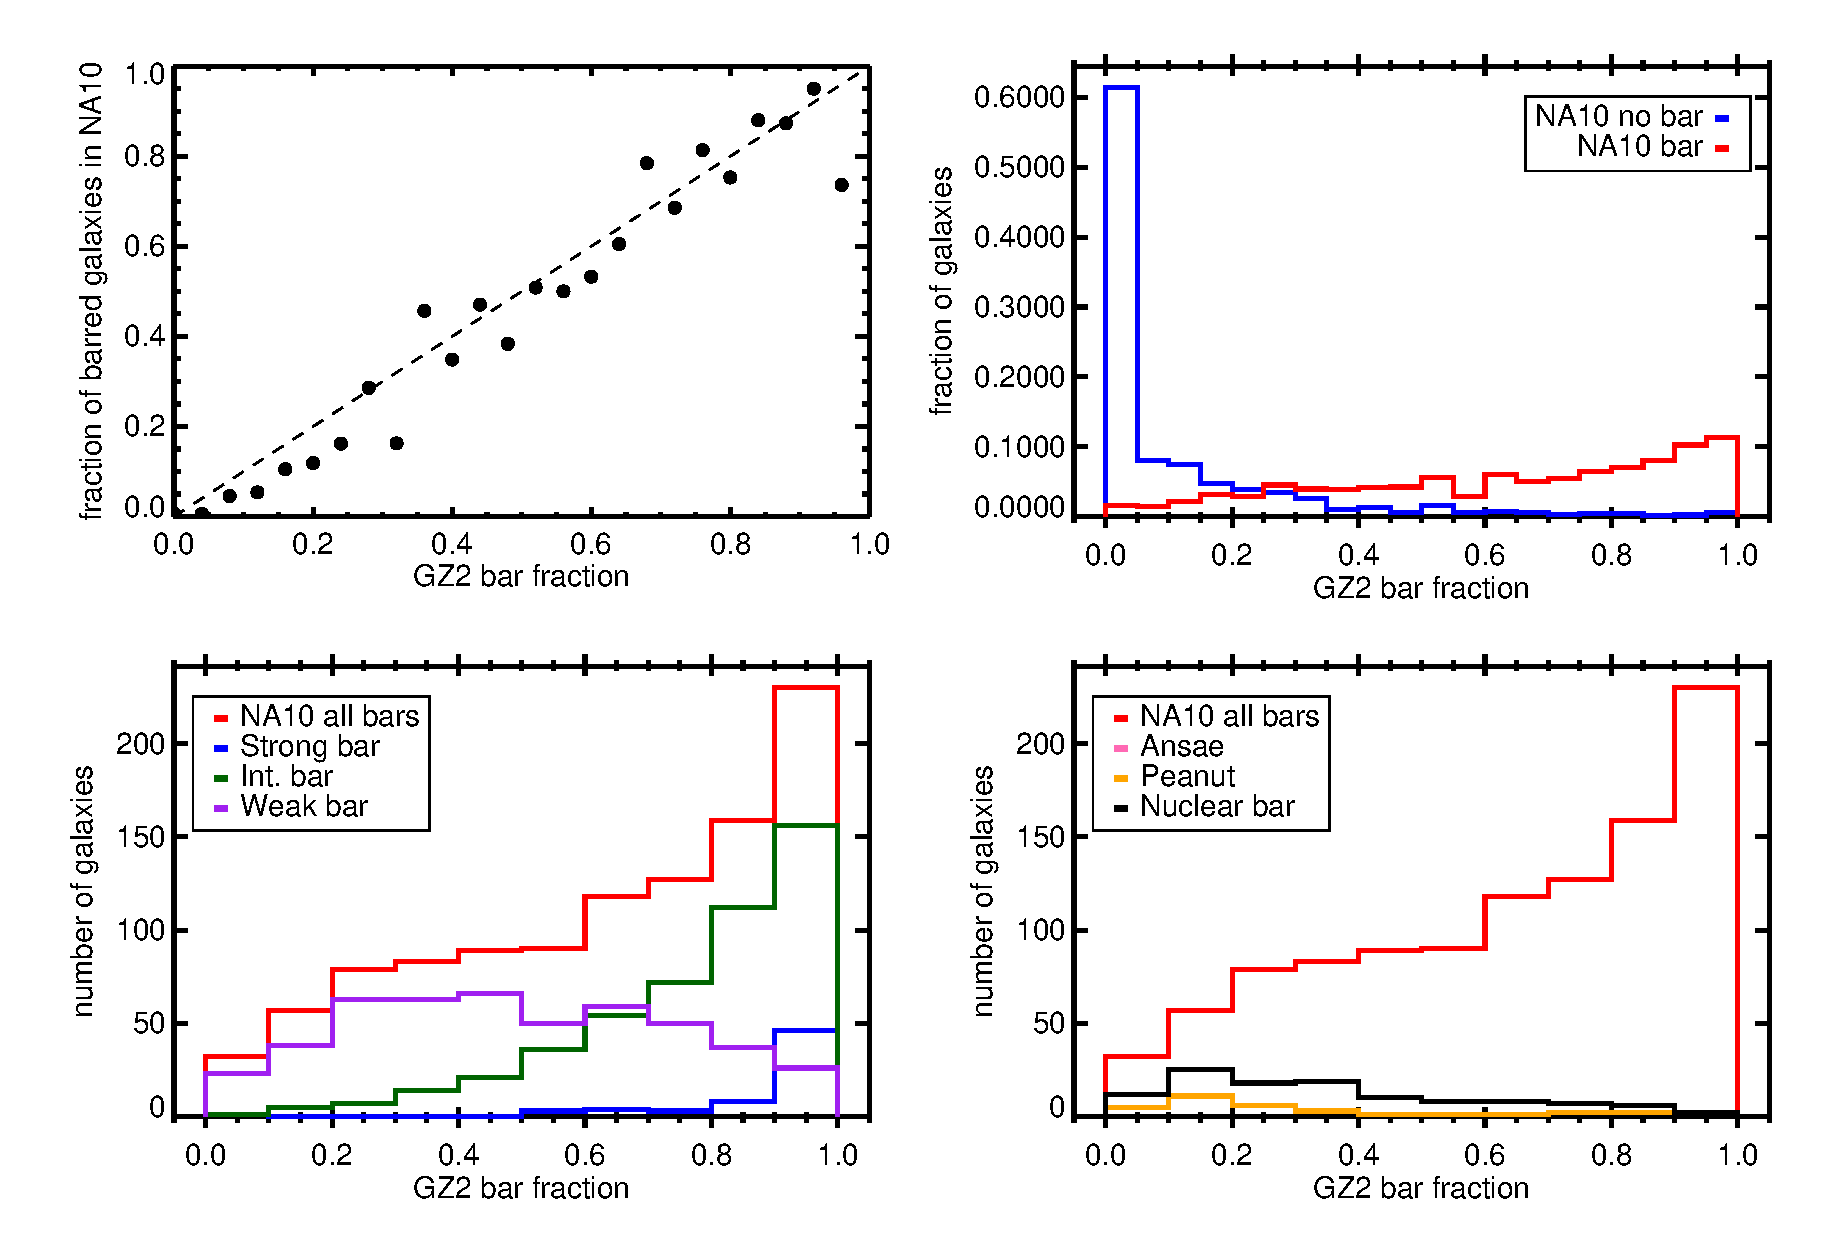
\includegraphics[angle=0,width=7.0in]{figures/na_bars_axial_10.eps}
\caption{Galactic bar classifications for GZ2 and NA10. Data are for the 7,121 galaxies which are face-on (log~$(a/b)<0.3$), have 10 or more GZ2 bar classifications, and appear in both samples. Top left: mean weighted bar fraction per galaxy in GZ2 vs. the ratio of barred to all galaxies in NA10 ({\it solid line}). Dashed line shows the one-to-one relationship. Top right: distribution of the GZ2 bar vote fraction, separated by NA10 classifications (including all bars). Bottom left: distribution of GZ2 bar vote fraction for the three disk-scale bar categories of NA10. Bottom right: distribution of GZ2 bar vote fraction for ansae, peanut, and nuclear bars in NA10. 
\label{fig-na_bars}}
\end{figure*}

The top right panel of Figure~\ref{fig-na_bars} shows the distribution of GZ2 bar votes by simply splitting the NA10 sample in two: galaxies without a bar and galaxies with a bar (of any kind). Both samples show a strong trend toward either extrema, with the strong peak near 0.0 for non-barred galaxies indicating that GZ2 classifiers are very consistent when no bar is present in the galaxy. Possession of a bar is less straightforward; while the frequency of NA10 bars does increase with GZ2 fraction, 32\% of NA10-barred galaxies have a GZ2 vote fraction $<0.5$. Conversely, there are very few false positives (5.5\% of non-barred NA10 galaxies) above this value. 

In the bottom left of Figure~\ref{fig-na_bars}, the distribution of GZ2 vote fraction as a function of NA10 bar strength is plotted. The distribution for all bars is the same as shown in the top right, increasing with GZ2 vote fraction. There is a clear difference in GZ classification between the three sets of bars; interestingly, all three are statistically highly distinct from each other and from the overall barred sample, according to a two-sided K-S test. The majority of both the strong and intermediate barred population have high GZ2 vote fractions, with 83\% of strong bars and 56\% of intermediate bars above a bar fraction of 0.8. Those numbers increase to 98\% and 90\%, respectively, if the criterion of 0.5 for the GZ2 vote fraction is used \citep{mas11c}. Weakly-barred galaxies have only 13\% of their GZ2 vote fractions above 0.8 and 47\% above 0.5. 

The lack of sensitivity to medium and weak bars (as IDed by NA10) may be due in part to the design of the GZ2 interface. When users are asked if a bar is present, they are presented with a simple pictogram showing two examples of a barred galaxy. For the pictogram showing a disk, the bar drawing extends across its full diameter, fitting with the typical definition of a strong bar. With this as the only example (and no continuum of options between the two choices), GZ2 users may not have looked for bars shorter than the disk diameter, or been less confident in clicking ``yes'' if they did see them. Results from \citet{hoy11} show that users are fully capable of identifying weak bars in other contexts; however, the construction of our decision tree means that GZ2 classifications only include examples from strong and medium bars. 

NA10 identify three other fine-structure features related to bars: ansae, peanuts, and nuclear bars. None of the three correlate strongly with the GZ2 bar parameter, with more galaxies actually having vote fractions $<0.5$ than above it. Nuclear bars are the only feature that overlaps with the NA10 bar strength classifications; out of 283 nuclear bars, 3 galaxies also have strong bars, 44 have intermediate bars, and 166 have weak bars. No ansae are detected in the GZ2 face-on subsample, likely due to our axial cut. 

In the GZ2 main sample, 15,873 galaxies are in the clean, debiased sample of bars (as set by the flag in the data). This is 29.6\% of the clean sample of face-on galaxies, in extremely good agreement with both the 29.4\% fraction found in the smaller volume-limited sample of \citet{mas11c}, and with the $\sim30\%$ for disk galaxies with $(b/a)>0.4$ (or log~$(a/b)<0.398$) and T-types of S0 or later of \citet{nai10a}. 

%In the published literature, \citep{mas11c} mention the NA10 catalog and note that both papers agree with a bar fraction depending on morphology with a minimum near the division between the blue and red sequences. There is no detailed comparison between the galaxies in the two samples.

\subsubsection{Rings}

NA10 also classifies ring galaxies in their catalog. They include three basic types of rings based on the \citet{but96} criteria. Inner rings lie between the bulge and spiral arms or disk. Outer rings are external to the spiral arms, but are still closely linked to the spiral pattern. Nuclear rings lie in the bulge region of galaxies; no specific size scale for this is given. In GZ2, rings are classified only if the user answers ``yes'' to the question {\it ``Anything odd?''} Since the user then has seven different options to choose from (ring, lens, disturbed, irregular, other, merger, dust~lane), interpreting the weighted ring fractions is less straightforward. 

In the NA10 catalog, 18.2\% of galaxies have a ring. Of those, 10\% are nuclear rings, 74\% are inner rings, and 32\% are outer rings (sum is more than 100\% since $\sim1/3$ of ringed galaxies have multiple rings flagged). In the GZ2 catalog, 3,142 galaxies are in the clean sample of rings, but this is based on only a potentially small number of total votes ($N\geq5$). In both catalogs, selecting only face-on galaxies did not significantly change the percentage of galaxies identified as having a ring. 

In the top-left of Figure~\ref{fig-na_rings}, the distribution of the number of GZ2 votes for a ring in face-on galaxies is shown, both for the total sample and for galaxies classified by NA10 as having a ring. The distributions grow closer as the number of ``yes'' votes increases. The top-right panel of Figure~\ref{fig-na_bars} shows the CDF for the number of ring votes. Among all galaxies with at least 15 ``yes'' votes, for example, $\sim90\%$ of those galaxies are also identified by NA10 as having a ring; almost all of these are inner or outer rings.  

\begin{figure*}
\includegraphics[angle=0,width=7.0in]{figures/na_rings_axial.eps}
\caption{Ring classifications in GZ2 and NA10. Data are for the 9,746 galaxies in both samples which are face-on (log~$(a/b)<0.3$). Top left: distribution of NA10 ringed galaxies compared to all face-on galaxies as a function of the raw number of votes for a ring in GZ2. Bottom right: distribution of NA10 ringed galaxies compared to all face-on galaxies as a function of the GZ2 vote fractions for ring. Top right: Fraction of face-on galaxies that have a ring (NA10) as a function of the total number of votes for a ring in GZ2. Bottom right: Fraction of face-on galaxies that have a ring (NA10) as a function of the GZ2 ring vote fraction. 
\label{fig-na_rings}}
\end{figure*}

The vote fraction for rings from GZ2 is not a good match to the ring classifications of NA10. Half of all galaxies have a vote fraction of 0.0, indicating no votes for a ring-like structure in the image. For ringed galaxies identified by NA, the number of galaxies with no GZ2 votes decreases dramatically, but results a generally flat distribution of ring fractions. No single cut on GZ2 vote fraction is a good proxy for the NA10 classifications; at $f<0.5$, for example, only $\sim45-65\%$ of the GZ2 ringed galaxies are identified as rings in NA10.  

There is some evidence indicating that GZ2 classifications are sensitive only to certain types of rings. NA10 galaxies with nuclear rings, for example, have a large number of galaxies with no GZ2 ring votes. Several causes are possible: since nuclear rings are smaller, they are more difficult to discern in low surface brightness or bulge-dominated galaxies. In addition, the button in the GZ2 tree intended to show an example of a ring has a centre dot (presumably a galactic bulge) surrounded by a ring. This could reasonably represent either an inner or outer ring, but would presumably not be associated with the intra-bulge nuclear rings by an untrained user. The bottom-right panel of Figure~\ref{fig-na_rings} shows that the number of NA10 galaxies with inner and/or outer rings does rise with vote fraction, but is still only 55\% successful at $f > 0.8$. 

\subsubsection{Mergers/interacting galaxies}

Galaxies in GZ2 can be labeled as a ``merger'' under the task {\it ``Anything odd?''} NA10 classify possible mergers in two ways: by identifying pairs of objects in an image, and by identifying interacting galaxies. Both NA10 categories have sub-levels: paired objects are sorted by relative separation (close, projected, apparent, or overlapping pairs), and interactions by morphology (disturbed, warp, shells, tails, or bridges). If tidal tails are present, there is an additional flag couting the number of tails. 

In the NA10 catalog, 22.3\% of galaxies are labeled as paired; of these, the majority (72\%) are close pairs. Interacting galaxies are a much smaller subset, comprising 7\% of the NA10 sample. In the GZ2 catalog, only 252 galaxies are in the clean sample identified as merging. If the vote totals for a possible merger are used instead, 5\% (3\%) of the NA10 paired galaxies have at least 5 (10) votes for a merger. The large fraction of NA10 galaxies suggests that this is less likely to be a good proxy for a merger as identified by the GZ2 votes. 

\begin{figure*}
\includegraphics[angle=0,width=7.0in]{figures/na_pairs.eps}
\caption{Merger classifications in GZ2 and NA10. Data are for the 12,480 galaxies in both samples. This includes all galaxies in the overlap sample (black), galaxies in pairs (blue), and interacting galaxies (red). Top left: distribution of NA10 paired galaxies compared to all galaxies as a function of the raw number of votes for a merger in GZ2. Bottom right: distribution of NA10 paired galaxies compared to all galaxies as a function of the GZ2 vote fractions for merger. Top right: Fraction of paired galaxies (NA10) as a function of the total number of votes for a merger in GZ2. Bottom right: Fraction of paired galaxies (NA10) as a function of the GZ2 merger vote fraction. 
\label{fig-na_pairs}}
\end{figure*}

Figure~\ref{fig-na_pairs} shows the distributions of NA10 paired and interacting galaxies. Most galaxies in the overlapping sample have no votes for a merger; the same trends are seen for both pairs and interactions. Using the raw number of votes as a cutoff, GZ2 galaxies stabilize at an 80\% match rate to the NA10 paired galaxies for 8 or more merger votes. The trend for interacting galaxies continues to increase with more votes, only matching the 80\% level at $>25$ votes, for which less than 100 galaxies are included.

Using the vote fraction instead of the raw vote shows no strong correlation with the NA10 classifications. Interestingly, both distributions do show peaks if a vote fraction cutoff of 0.5 is chosen. The peak of the NA10 fraction, however, is significantly lower if matching on the vote fraction; only 70\% for paired galaxies and 40\% for interacting galaxies. This shows no difference depending on the type of NA10 pair. Within the NA10 interacting classes, all actually show a decrease in number for a higher vote fraction; the lone exception is galaxies classified by NA10 as ``bridges'', the fraction of which increases slightly above a GZ2 vote fraction of 0.5. 

Similar to the results for paired galaxies, there is no strong correlation between either the GZ2 vote fraction or number of merger votes and the number of NA10-identified tidal tails. 

{\em Merits further discussion of results in \citet{cas13}; perhaps KC can write a paragraph or two?}

\subsubsection{T-types}

There has been no published discussion in the literature comparing large-scale morphologies of the NA10 and Galaxy~Zoo catalogs. \citet{nai10} was published after the first GZ1 results \citep{lin08}, but prior to the formal data release paper \citep{lin11}. \citet{hue11} do compare automated classifications to both NA10 and GZ1, finding good agreement with both; this obliquely suggests that the GZ2 and NA10 classifications will also be consistent. 

The left panel of Figure~\ref{fig-na_ttype} shows the percentage of galaxies identified as having either a disk or features from the first question in the GZ2 tree, colour-coded by their NA10 T-types. There is a clear separation in the GZ2 fractions for galaxies classified as E vs. those with T-types Sa and later. Late-type galaxies, including S0's, have a median weighted fraction of the ``features or disk question'' of 0.796, with a standard deviation of 0.29. This distribution is bimodal, with one peak near 0.95 and a second at 0.1. Breaking down the late-type galaxies into more specific Hubble classifications, the late-type galaxies with low GZ2 feature votes are found to be primarily lenticular (S0; T-type = $-3$ to 0) galaxies. If only galaxies with T-types Sa or later are considered, the peak at lower GZ2 fractions disappears. The median GZ2 weighted fraction for these galaxies is 0.88, with a standard deviation of 0.23. The highest GZ2 weighted fraction for an elliptical galaxy in NA10 is 0.741; therefore, any cut above this limit includes {\it exclusively} identified by NA10 as late-type. Even if the confidence of this decreases for the larger GZ2 sample due to the inclusion of fainter galaxies, the previous limit of 0.8 (which may be conservative) reproduces the broad morphological cuts of NA10 extremely well. 

\begin{figure*}
\includegraphics[angle=0,width=7.0in]{figures/na_ttype.eps}
\caption{T-type classifications for NA10 and GZ2. Data in the left panel are for the 12,480 galaxies found in both samples; the right panel only shows the 5,683 galaxies with at least 10 responses to Task 04 (visible spiral structure) in GZ2. The distribution is of GZ2 weighted vote fractions separated by their T-type classification from NA10. 
\label{fig-na_ttype}}
\end{figure*}

Since there are very few objects identified as stars or artifacts in the first GZ2 question, the weighted fraction for smooth galaxies is approximately $f_{smooth} = (1 - f_{features/disk})$. Elliptical galaxies (T-type = $-5$) have a median weighted fraction of the ``smooth'' question of 0.86, with a standard deviation of 0.07. The GZ2 votes for the NA10 ellipticals are much more sharply peaked than the late-type galaxies, lacking the long tail seen even for very late types. This means that a cut on GZ2 votes for smooth galaxies at 0.8, for example, would include 4\% late-type galaxies (20\% if S0 galaxies are included). 

For galaxies identified as having features that are not edge-on disks, GZ2 users then vote on whether the galaxy has visible spiral structure (Task 04). For the few NA10 elliptical galaxies that have votes for this question, $\sim85\%$ of them have GZ2 weighted fractions of 0.0, with the remainder weakly clustered around 0.3. For NA10 late-type galaxies, the majority of disk/feature objects have high GZ2 spiral structure weighted fractions. For galaxies with at least 10 votes on Task 04 (a peak at 0.0 appears when this cut is not imposed), 70\% of Sa or later-types have a GZ2 spiral vote fraction $>0.8$. This drops to 60\% if S0 galaxies are included as late-type. The missing population is thus made up of galaxies with significant spiral structure by NA10, but for which GZ2 users cannot distinguish spiral arms. One might expect these galaxies to have lower magnitudes or surface brightnesses compared to the rest of the sample, thus lowering the confidence of GZ2 votes (there is no analog parameter associated with NA10 classifications). However, the apparent $g$ and $r$ magnitudes, as well as the absolute $g$-band magnitude, show no difference between galaxies above and below the 80\% cutoff. Experimenting with other values for the GZ2 weighted fraction had no change on the results.  

\subsubsection{Spiral tightness}

\begin{figure*}
\includegraphics[angle=-90,width=7.0in]{figures/spiraltightness_color.ps}
\caption{T-type classifications compared to the GZ2 vote fractions for spiral tightness (Task 10). Left side is NA10 T-types; right side is EFIGI T-types. Data are for the 5,515 (NA10) and 1,907 (EFIGI) galaxies, respectively, with at least 10 GZ2 votes for Task 10. The number of galaxies per bin is given along the top of each panel. 
\label{fig-spiraltightness}}
\end{figure*}

If a disk galaxy was identified as having spiral structure, Task~10 in GZ2 asked users to classify the ``tightness'' of the arms. This had three options: tight, medium, or loose (accompanied with pictograms on buttons that illustrated representative pitch angles). This has direct (but not exclusive) connections to the Hubble classification of late-type galaxies; tight spirals would be Sa/Sb, medium spirals Sb/Sc, and loose spirals Sc/Sd. The agreement between the GZ2 classification can be compared to Hubble types by using the NA10 classifications. 

The left side of Figure~\ref{fig-spiraltightness} shows the distribution of NA10 T-types for galaxies based on their GZ2 weighted fractions for winding arms. This figure shows only galaxies with at least 10 votes on spiral structure; looking at all galaxies in the overlapping sample disproportionally weights the 0.0 and 1.0 weighted fraction bins. Weighted fractions for both tight and medium winding arms are relatively normally distributed, with tight spirals peaking near 0.46 and medium spirals at 0.37. Strongly-classified loose spirals are much rarer, with 75\% of galaxies having a weighted fraction of less than 0.2. Almost no elliptical galaxies from the NA10 catalog are included, although there are significant numbers of S0 galaxies. 

For tight spirals, galaxies with the highest weighted fractions have more earlier-type spirals than galaxies with a low vote for tight spiral winding arms. For a tight spiral weighted fraction above 0.9, 85\% of galaxies are Sb or earlier. Medium-wound spirals with high weighted fractions tend to be Sb and Sc galaxies -- the proportion of both types increases as a function of medium-wound weighted fraction, and constitute 84\% of galaxies when the weighted fraction is greater than 0.6. Galaxies strongly classified as medium-wound are rare, however, with only 23 galaxies having a weighted fraction above 0.8.  Loose spirals are dominated by Sc and Sd galaxies at high weighted fraction values, comprising more than 50\% of galaxies above a loose weighted fraction of 0.7. 

Overall, we see a clear trend for looser GZ2 spiral arms to correspond with later spiral T-types from NA10 classifications. High weighted vote fractions are mostly Sa/Sb galaxies for tight winding, Sb/Sc galaxies for medium winding, and Sc/Sd galaxies for loose winding. Individual GZ2 vote fractions, however, have significant diversity even at the highest bins, and do not reliably separate the morphologies on the level of the Hubble T-types. 

%It would be potentially useful to try combining the winding arms classifications to improve the 40\% false positive rate; for example, by seeing if a high value for loose weighted fraction + a low value for a tight weighted fraction increased the fraction of Sc and Sd galaxies in the highest bins. 

\subsubsection{Bulge dominance}

\begin{figure*}
\includegraphics[angle=-90,width=7.0in]{figures/bulgeprominence_color.ps}
\caption{T-type classifications compared to the GZ2 vote fractions for bulge prominence (Task 05). Left side is NA10 T-types; right side is EFIGI T-types. Data are for the 7,120 (NA10) and 2,321 (EFIGI) galaxies, respectively, with at least 10 GZ2 votes for Task 05. The number of galaxies per bin is given along the top of each panel. 
\label{fig-bulgeprominence}}
\end{figure*}

\begin{figure}
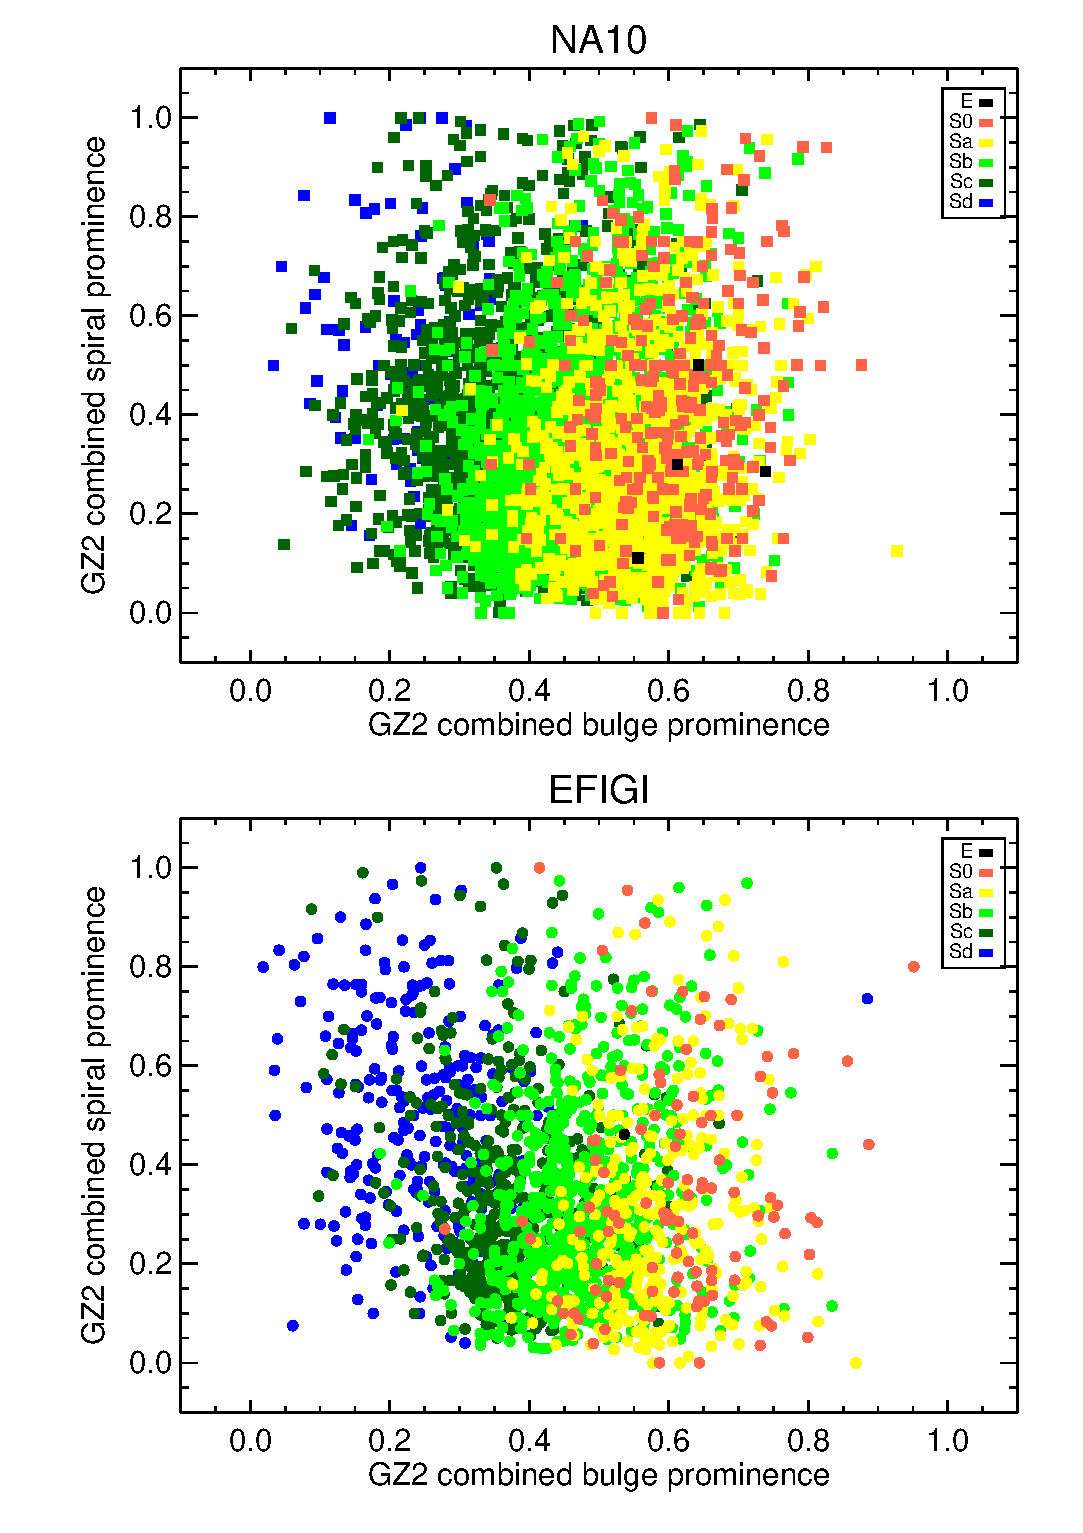
\includegraphics[angle=0,width=3.3in]{figures/wbulge_wspiral.eps}
\caption{Weighted bulge classifications vs. weighted spiral classifications from GZ2. Galaxies are colour-coded by their morphologies in EFIGI ({\it top}) and NA10 ({\it bottom}). Data are for galaxies with at least 10 classifications for both Task 05 (bulge dominance) and Task 10 (spiral structure) in GZ2. 
\label{fig-bulgespiral}}
\end{figure}

Disk galaxies in GZ2 are also classified by the visible level of bulge dominance (Task~05), irrespective of whether spiral structure is also identified. This task has four options: ``no bulge'', ``just noticeable'', ``obvious'', and ``dominant'' (accompanied with pictograms that illustrated bulge sizes compared to face-on spiral arms). Similar to the arm tightness task, we analyze the relationships between GZ2 classification and Hubble types from NA10. 

The left side of Figure~\ref{fig-bulgeprominence} shows the distribution of NA10 T-types for galaxies based on their GZ2 weighted fractions for winding arms. This figure shows only galaxies with at least 10 votes on bulge prominence. Weighted fractions for both the ``no bulge'' and ``dominant'' responses peak strongly near zero and tail off as the vote fraction increases. Responses to the middle options, ``just noticeable'' and ``obvious'', resemble normal distributions peaking near 0.5. 

``No bulge'' galaxies in GZ2 are dominated by Sc and Sd spirals for non-zero weighted fractions. For weighted fractions above 0.1, 81\% of galaxies are Sc or later; this rises to 100\% for weighted fractions higher than 0.6. ``Just noticeable'' galaxies show a smooth change in T-type distribution; low weighted fractions are dominated by S0 and Sa galaxies, while high weighted fractions are Sb--Sd. ``Obvious'' bulge galaxies are almost a mirror image of the ``just noticeable'' votes; low weighted fractions are Sb--Sd galaxies, and high weighted fractions are S0--Sa galaxies. Among galaxies classified as ``dominant'', less than 10 galaxies have weighted fractions above 0.6 (which are a surprisingly diverse mix of S0, Sa, and Sd). Most remaining galaxies have dominant weighted fractions of less than 0.1; the T-types of the remaining galaxies between 0.1 and 0.6 mostly contain S0 and Sa spirals. 

The link to T-type is more sharply defined for bulge prominence than for spiral tightness, according to the NA10 classifications. Very clean samples of late-type (Sb--Sd) spirals can be selected using only the ``no bulge'' parameter; additional samples with $\sim10$\% contamination can be selected with the ``just noticeable'' and ``obvious'' distributions. Early-type spirals and lenticulars at the same purity level can also be selected. Elliptical galaxies for which the bulge question was answered are most often ``dominant'', but there is no obvious separation of ellipticals from disk galaxies based on this task. 

Since Hubble types are based on both bulge dominance and the distance of their spirals, we explore whether the combination of Tasks 05 and 10 from GZ2 improve the separation between T-types. Figure~\ref{fig-bulgespiral} shows the GZ2 bulge prominence vs. spiral tightness, colour-coded by their NA10 T-types. The GZ2 variables are simple weighted averages of the vote fractions for all possible task responses, where:

\begin{eqnarray}
\label{eqn-wbulge}
\omega_{bulge} = (0f_{nobulge} + 1f_{justnoticeable} \\
            + 2f_{obvious} + 3f_{dominant}) / 3., \nonumber
\end{eqnarray}

\noindent and 

\begin{equation}
\label{eqn-wspiral}
\omega_{spiral} = (0 \times f_{tight} + 1 \times f_{medium} + 2 \times f_{loose}) / 2.
\end{equation}

Using the weighted feature classifications shows a clear separation in T-types; the majority of this, however, is for the bulge prominence category. Spiral prominence does not seem to significantly affect any of the classifications.

Finally, we note that \citet{sim13} identified a significant effect in which nuclear point sources, such as AGN, can mimic bulges in the GZ2 classifications. This has not yet been accounted for in this analysis, but could potentially be addressed by separating the sample into AGN and quiescent galaxies (via BPT line ratios) and looking for systematic differences between the two samples. 

%\subsubsection{T-types to clicks}
%
%\begin{itemize}
%	\item How like a given T-type is a galaxy?
%	\item Take all GZ2 vote fractions, plus galaxy metadata ($z, R_{50}, m_R, \mu$)
%	\item Run a PCA on NA10 classifications to see which GZ2 parameters are most important
%	\item Apply it and get the likelihood of a particular galaxy from the ~20 axes
%	\item This is the training set that is applied to the rest of Zoo2, accounting for evolution in the metadata properties on which the PCA can act.
%\end{itemize}

\subsection{EFIGI}

\citet{bai11} performed individual morphological classifications of 4,458 galaxies for EFIGI (Extractions de Formes Id\'ealis\'ees de Galaxies en Imagerie). The sample is a subset of the RC3 catalog for which 5-colour imaging in the SDSS DR4 was available. Images are supplemented by redshift information from several different sources. The galaxies have no strong redshift or volume limit on the sample, with almost all galaxies at $0.0001<z<0.08$. Classifications on composite $gri$ images were performed by a group of 11 salaried astronomers, each of whom classified a subset of 445 galaxies. A training set of 100 galaxies was also classified by all astronomers in the group to adjust the sample for individual bias. 

EFIGI contains two types of morphological classification: T-types and attributes. T-types are assigned using a slightly modified version of the RC3 Hubble classifications. Peculiar galaxies are not considered a separate stage, and ellipticals are subdivided into various types: compact, elongated (standard elliptical), cD (giant elliptical), and dwarf spheroidals. They also classify late-type lenticulars (S0$^+$; T-type=$-1$) that are not included in the classification of NA10. The remaining morphological information, called attributes, is divided into six groups:

\begin{itemize}
	\item appearance: {\tt inclination/elongation }
	\item environment: {\tt multiplicity, contamination}
	\item bulge: {\tt B/T ratio}
	\item spiral arms: {\tt arm strength, arm curvature, rotation}
	\item texture: {\tt visible dust, dust dispersion, flocculence, hot spots}
	\item dynamics: {\tt bar length, inner ring, outer ring, pseudo-ring, perturbation}
\end{itemize}

\noindent Attributes are defined on a five-step scale from 0 to 1 (0, 0.25, 0.50, 0.75, 1) that describe the strength of the feature in question. For some attributes (eg, arm strength, rings), the scale is set by the fraction of the flux contribution of the feature relative to that of the entire galaxy; this scale may not be linear. For others (eg, inclination or multiplicity), it ranges between the extrema of possible values. A 70\% confidence interval (roughly 1$\sigma$) is estimated by setting lower and upper limits on the same five-point scale.

EFIGI is compared in detail to NA10 in \citet{bai11}. Only $\sim10\%$ of the NA10 catalog overlaps with EFIGI classifications; roughly one-third of the EFIGI sample lies at redshifts below the NA10 lower limit of $z=0.01$, and also contain significant number of galaxies fainter than $g=16$. T-types agree well between the two samples; EFIGI lenticular and early spirals have slightly later average classifications in NA10, while later EFIGI galaxies have slightly earlier NA10 T-types. EFIGI has a major fraction of galaxies with slight-to-moderate perturbations that have no interaction flags in the NA10 catalog, indicating that NA10 is less sensitive toward more benign features (eg, spiral arm asymmetry). The bar length scale is consistent between the two samples; good agreement is also found for ring classifications. 

3,411 galaxies appear in both EFIGI and GZ2. This constitutes 77\% of the EFIGI galaxies and 1.2\% of the GZ2 sample. Like NA10, it offers a supervised set for comparisons between citizen scientists and salaried astronomers. The comparisons also benefit (or possibly detract) from the fact that EFIGI, like GZ2, has multiple classifiers and thus possible variance based on individual bias. 

\begin{figure*}
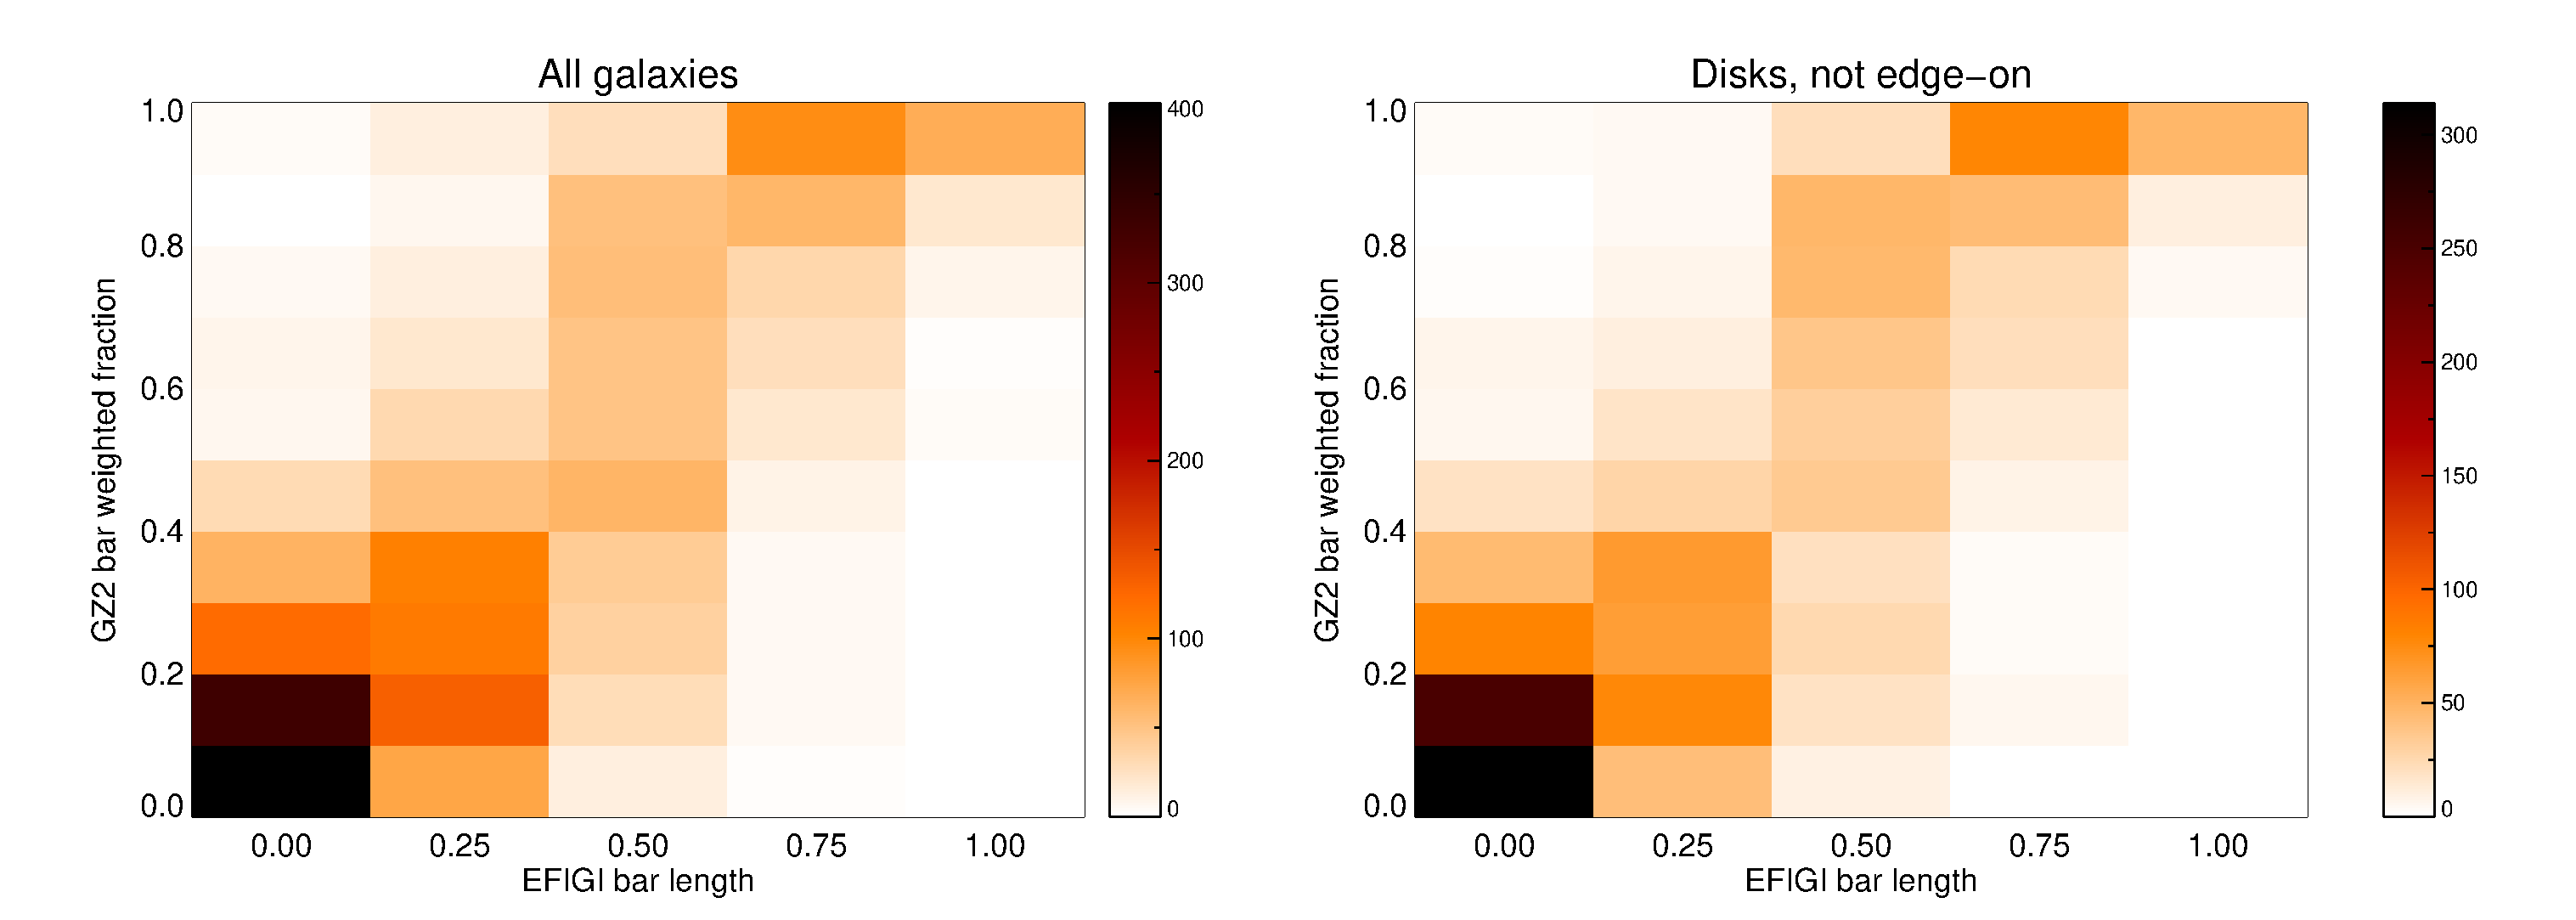
\includegraphics[angle=0,width=7.0in]{figures/efigi_bars.eps}
\caption{EFIGI bar length classifications compared to their GZ2 weighted fractions for the presence of a bar. Data on the left are for the 3,354 galaxies in both samples; the subset of 2,099 face-on galaxies is on the right. The dashed line is not a fit to the data, but is the one-to-one correlation. 
\label{fig-efigi_bars}}
\end{figure*}

\subsubsection{Bars}

GZ2 asks users to identify whether a bar is present in the galaxy. EFIGI's scale is based on bar length (not necessarily corresponding to strength) with respect to $D_{25}$, the decimal logarithm of the mean isophote diameter at a surface brightness of $\mu_B=25$~mag~arcsec$^{-2}$. A value of 1.0 (the strongest bar) extends more than half the length of $D_{25}$, while the median value of 0.5 would be about one-third the length of $D_{25}$. 

There is a strong correlation between the GZ2 weighted fractions for bars and the bar attribute strength from EFIGI (Figure~\ref{fig-efigi_bars}). 65\% of GZ2 galaxies in the overlap sample have no strong evidence for a bar (less than 0.3); of those, 77\% had EFIGI bar attributes of 0.0 and 94\% had 0.25 or less. For higher values of the GZ2 bar weighted fraction, the EFIGI attribute is slightly lower; the largest number of galaxies with GZ2 weighted fraction above 0.8 have EFIGI values of 0.75. The correlation coefficient between the variables is 0.51; if only face-on galaxies are considered, this increases to 0.75. 

If the \citet{mas11c} GZ2 weighted fraction of $\geq0.5$, at least 10 bar votes, and face-on galaxies is applied, then 98\% (646/660) galaxies overlapping with the EFIGI catalog have a bar attribute above 0. The mean EFIGI attribute (weighted by the confidence intervals) for galaxies barred by the \citet{mas11c} criteria is 0.62, indicating a selection preference toward medium-length bars, between one-third and one-half of $D_{25}$. 

The overall fraction of barred galaxies in EFIGI is 42\% (1439/3354); this is essentially unchanged if only face-on galaxies are considered (915/2099 = 44\%). This is significantly higher than the mean bar fraction of \citet{mas11c}, at 29.5\%, but consistent with results using automated ellipse-fitting techniques \citep{bar08,agu09}. The higher fraction in EFIGI is due to the contributions of galaxies with bar length attributes of 0.25, the majority of which have GZ2 weighted fractions below 0.5. If only EFIGI galaxies at 0.5 and above are considered to be barred, then the bar fraction falls to 17\%. Only some of the galaxies in the 0.25 EFIGI bin are being classified by the GZ2 users as barred; since \citet{bai11} defines this as a ``barely visible'' bar, it may be expected that less than half of GZ2 users would have detected it. 

\citet{mas11c} suggest in their paper that trends of bar fraction should ideally be discussed in the context of large or strong bars; an EFIGI cut of 0.5 or above would likely suit this philosophy best. 

It should also be noted that neither \citet{hoy11} nor \citet{bai11} compare the bar lengths derived using their separate methods, possibly due to their near-simultaneous publication. Since the bar catalog is publicly available, this can be done fairly easily, although it may not be appropriate for inclusion in this paper. 

\subsubsection{Arm curvature}

\begin{figure*}
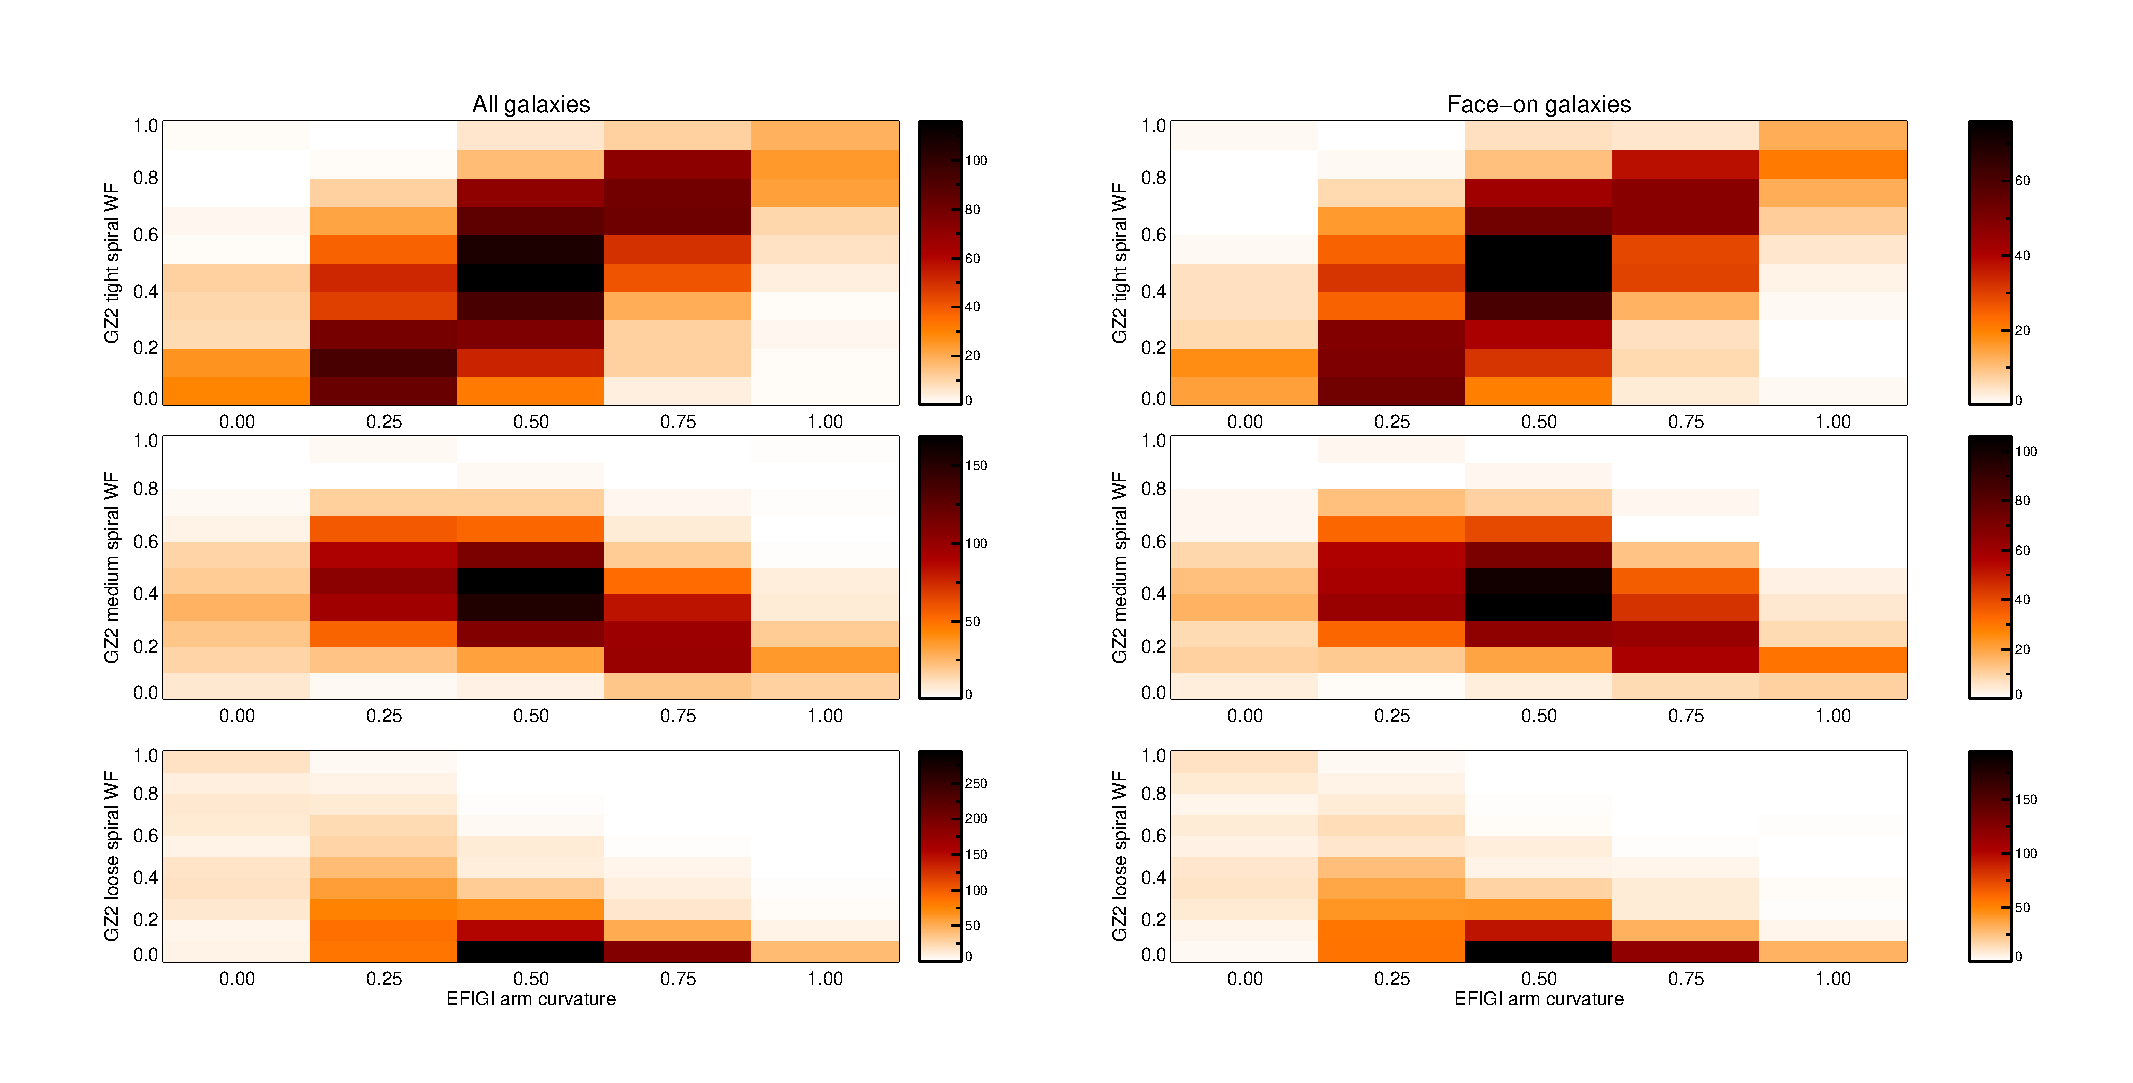
\includegraphics[angle=0,width=7.0in]{figures/efigi_arm_curvature.eps}
\caption{EFIGI arm curvature classifications compared to their GZ2 weighted fractions for the presence of a bar. Data on the left are for the 3,411 galaxies in both samples; the subset of 2,099 face-on galaxies is on the right. Dashed lines on the top and bottom pairs of plots show the one-to-one correlation, a Gaussian with $\mu=0.5$ and $\sigma=0.25$, and the one-to-one anti-correlation, respectively. 
\label{fig-efigi_arms}}
\end{figure*}

EFIGI measures the arm curvature of each galaxy, with classifications very similar to the ``tightness of spiral arms'' question (Task 10) in GZ2. If both tasks and classifiers agree, one would expect galaxies with high GZ2 weighted fractions/votes for tight spirals to have EFIGI classifications at 0.75--1.0; GZ2 galaxies classified as medium spirals to be centred around 0.5; and loose spirals to have arm curvatures of 0.0--0.25. 

The EFIGI arm curvature classifications broadly follow the trends expected from matching targets with GZ2. The tight spiral weighted fraction follows the trend of the EFIGI arm curvature (Figure~\ref{fig-efigi_arms}). The Spearman's correlation coefficient for tight spirals is $\rho=0.62$. The medium spiral weighted fraction is clustered in the middle of the EFIGI values, where galaxies with the highest GZ2 weighted fraction have EFIGI values of 0.25--0.50, with $\rho=-0.26$. Loose spirals shows an anti-correlation ($\rho=-0.54$); very few galaxies have GZ2 weighted fractions above 0.5, but those which do have low EFIGI arm curvature values (0.0--0.25). 

Trends described above are quantitatively similar for both the full matching sample and for face-on galaxies only (right side of Figure~\ref{fig-efigi_arms}). Somewhat surprisingly, the distribution also appears similar if only considering galaxies with a mininum number of GZ2 votes on spiral winding arms. Lower limits of 5, 10, 20, and 30 votes produce the same patterns for all three categories. The correlation coefficient for both tight and medium spirals does decrease to $|\rho<0.2|$ if a 10-vote lower limit is applied. 

Notes:
\begin{itemize}
\item Most useful: look at high weighted fractions and high numbers of vote counts for the spiral winding category of choice. That might correlate most strongly with EFIGI values. 

\item EFIGI values are matched to specific pitch angles of the galaxy. For galaxies in which the GZ2 WF does not match the EFIGI, what is happening? Are the vote categories laterally skewed, are we not sensitive to weakest spirals, or is something else going on?

\item Not convinced that the face-on criterion is working. 

\item Change bar plot to single-panel version. Change right side of arm curvature to cuts on count and weighted vote fraction, show stronger correlations. Discuss the percentage of the total number of galaxies that this constitutes for the expanded GZ2 sample, and how many ``clean'' galaxies from the EFIGI criteria we might be able to extract (subject to bias at lower surface brightnesses).
\end{itemize}

\subsection{Huertas-Company -- automated classifications}

\begin{figure*}
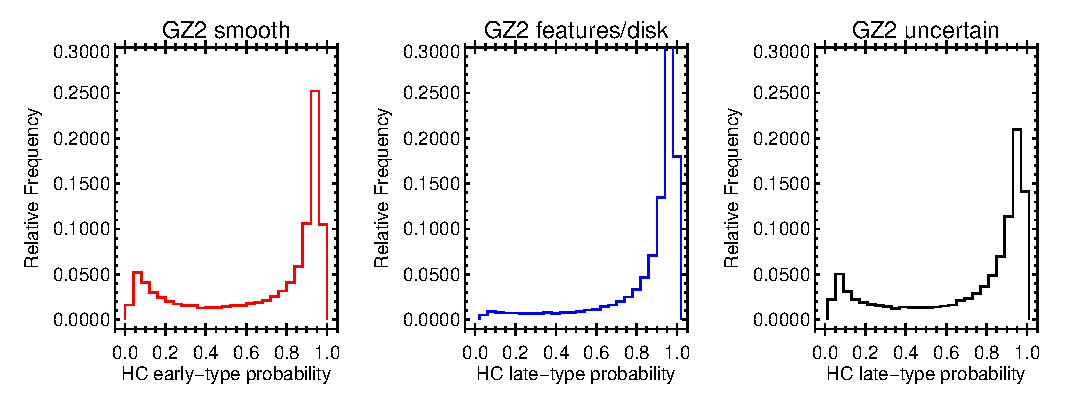
\includegraphics[angle=0,width=7.0in]{figures/hc_histogram.eps}
\caption{Left: distribution of HC early-type probabilities for galaxies with Task 01 ``smooth'' weighted fraction above 0.8. Middle: distribution of HC late-type probabilities for galaxies with Task 01 ``features or disk'' weighted fraction above 0.8. Right: HC late-type probabilities for uncertain galaxies ($p<0.8$ for all responses to Task 01). 
\label{fig-hc_histogram}}
\end{figure*}

\citet[][HC]{hue11} published a study in which they used training sets of galaxy images to create automated classifications, and then compared the results to GZ1. There have been no comparisons to GZ2; however, the broad nature of their probabilities (four broad morphological categories) largely unsuited for the fine structure questions such as bar and spiral number. 

The sample of galaxies classified by HC is the SDSS DR7 spectroscopic sample, limited to galaxies with $z<0.25$ with good photometric data and clean spectra. Their total of 698,420 galaxies is approximately twice the size of the GZ2 sample, which has a similar redshift range. The HC sample goes to fainter magnitudes, with more than 400,000 galaxies below the GZ2 limit of $r>17$. Their algorithm is implemented using support vector machine software that tries to find boundaries between points in $N$-dimensional space, where $N$ is determined by criteria including morphology, luminosity, colour, and redshift \citep{hue08}. The training set is the 2,253 galaxies in \citet{fuk07}, which have already classified by T-type. Each galaxy is assigned a probability of being in one of four subclasses: E, S0, Sab, and Scd (the latter two combine their two respective late-type categories). 

\citet{hue11} directly compare their results to the GZ1 sample from \citet{lin11}. They find that robust classifications in GZ1 (flagged in our clean sample as being either confirmed ellipticals or spirals) have median probabilities of 0.92 according to their algorithm, indicating that sure GZ1 classifications are also sure in their catalog. They also find a (but not strictly linear) relationship between the GZ1 debiased vote fraction and the HC probabilities. This is one of the first independent confirmations that the vote fractions may be related to the actual {\em probability} of a galaxy possessing a particular morphology. 

HC also compare their results to the NA10 data, most of which are not included in the HC training sample. They find a good correlation between the NA10 T-types and the HC probabilities, especially for ellipticals and Scd spirals. S0 galaxies are more difficult to separate; for the NA10 lenticulars, HC11 give only a 0.4 probability of S0, with 0.32 of elliptical and 0.2 of being Sab. Sab galaxies have an average probability of 0.55 being an Sab in HC, but also 0.15 of being S0 or Scd. The HC algorithm is thus very good at identifying galaxies at the extreme ends of the Hubble tuning fork, but have larger amounts of overlapping probabilities for intermediate states. 

Since the GZ2 galaxies are a subset of the GZ1 sample, the results for Task~01 are expected to be similar to those described in \citet{hue11}. Figure~\ref{fig-hc_histogram} shows the distributions of the HC early- and late-type probabilities for GZ2 galaxies robustly identified ($f>0.8$) as either smooth or having features/disks. The median HC early-type probability for GZ2 ellipticals is 0.85, and the late-type probability for GZ2 spirals is 0.95. This confirms the result that robust classifications in Galaxy~Zoo agree with the automated algorithm. 

An exception to this is a population of galaxies classified as ``smooth'' by GZ2 users, but which have very low early-type probabilities from HC (the bump on the left side of the first panel in Figure~\ref{fig-hc_histogram}). The mean GZ2 vote fraction for these galaxies is consistent with those with high early-type probabilities -- these galaxies are not marginally classified as ellipticals in GZ2. The roundness of the galaxy (Task~07 in GZ2) seems to play some role, as the low-HC smooth galaxies have fewer round galaxies and many more ``cigar-shaped'' galaxies in this sample. A high axial ratio might have trained the HC algorithm to infer the existence of a disk; the absence of any obvious spiral features or bulge/disk separation (verified by eye in a small subsample of the imaages) lead GZ2 users to categorize them as ``smooth''. There is a clear dependence on apparent magnitude; the lower peak disappears if only galaxies with $r<16$ are plotted. The lower peak is also significantly bluer than the higher peak, with respective colours of $(g-r)=0.67$ and $(g-r)=0.97$. Since the SVM method does include SDSS colours as a parameter, we conjecture that the low HC early-type probability is in part due to the fact that they are blue, in addition to morphological features such as shape and concentration. It would be interesting to see what fraction of the blue ellipticals \citep{sch09} fall in this peak. 

The right panel of Figure~\ref{fig-hc_histogram} shows the distribution of ``unclassified'' galaxies, for which none of the reponses for Task 01 had a vote fraction $>0.8$. The HC probability for these galaxies is bimodal, with the larger fraction classified as HC late-type and a smaller fraction as HC early-type. 

Figure~\ref{fig-hc_gz2} plots the HC probability values against the GZ2 vote fraction for both smooth and feature/disk galaxies, similar to Figure~8 in \citet{hue11}. Significant excesses are seen at the lower left and upper right corners for both samples, confirming the earlier result that robust classifications using both methods tend to agree. The relationship of the HC probability to GZ2 vote fraction, however, seems distinctly non-linear and significantly different from the relationship shown in \citet{hue11}. Galaxies with low HC early-type probabilities show no strong correlation with the GZ2 weighted fraction, resulting in the vertical stripe in Figure~\ref{fig-hc_gz2}. Intermediate values of the HC probabilities are typically classified by GZ2 users as ``smooth'', with a concentration at the highest HC early-type probabilities. It should be noted that without GZ2 debiasing, the two panels in Figure~\ref{fig-hc_gz2} are essentially mirror images of each other (since $p_{HC,early} + p_{HC,late} \equiv 1$ and the GZ2 weighted fractions only have marginal contributions from either the star/artifact response or downweighting of inconsistent users). 

Splitting the morphology types into the E, S0, Sab, and Scd subclasses, Figure~\ref{fig-hc_gz2_subclass} shows correlations between the HC probablilities and GZ2 vote fractions. While the direction of the correlation is the same as seen in Figures~9 and 10 in \citet{hue11}, the behavior at the extrema is quite different. The debiased GZ1 data shows a strong cluster of low-HC and low-GZ probabilities for all four subclasses; no such cluster is seen in any of the plots in Figure~\ref{fig-hc_gz2_subclass}. Furthermore, high HC probabilities have the lowest fraction of galaxies in the GZ1 published data, where our plots show a concentration of galaxies along the high end for both P(E) and P(S0). It should be investigated whether the scaling on these sets of figures is truly plotting the same value. 

To do:
\begin{itemize}
	\item Check how the presence of a bar affects the HC classifications.
	\item Analyze the HC T-type vs. GZ2 bulge prominence (Figure~\ref{fig-hc_gz2_bulge_contour}).
\end{itemize}

\begin{figure*}
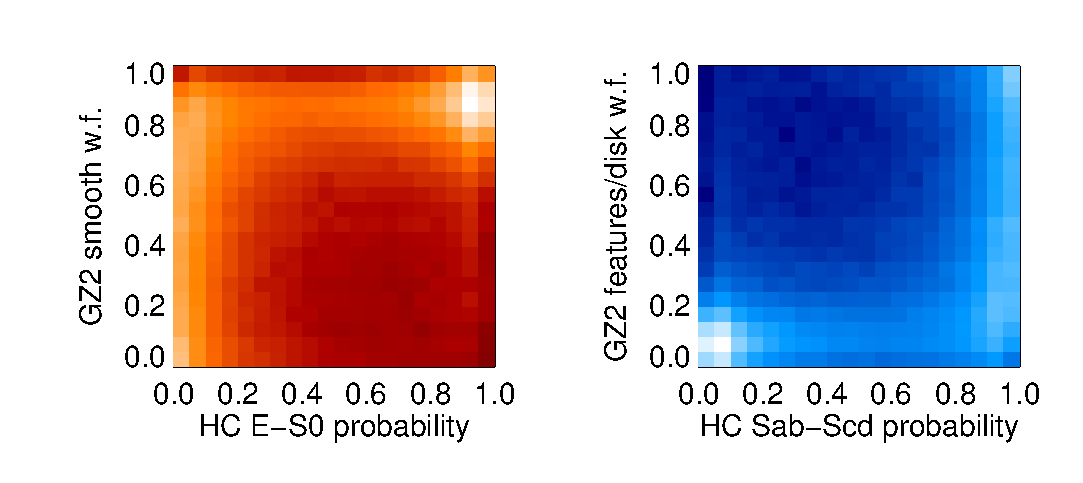
\includegraphics[angle=0,width=7.0in]{figures/hc_gz2.eps}
\caption{Left: GZ2 smooth weighted fraction as a function of \citet{hue11} early-type probability. Right: GZ2 features/disk weighted fraction as a function of HC late-type probability. Whiter values in both indicate a larger fraction of galaxies in that bin (logarithmic scale).
\label{fig-hc_gz2}}
\end{figure*}

\begin{figure*}
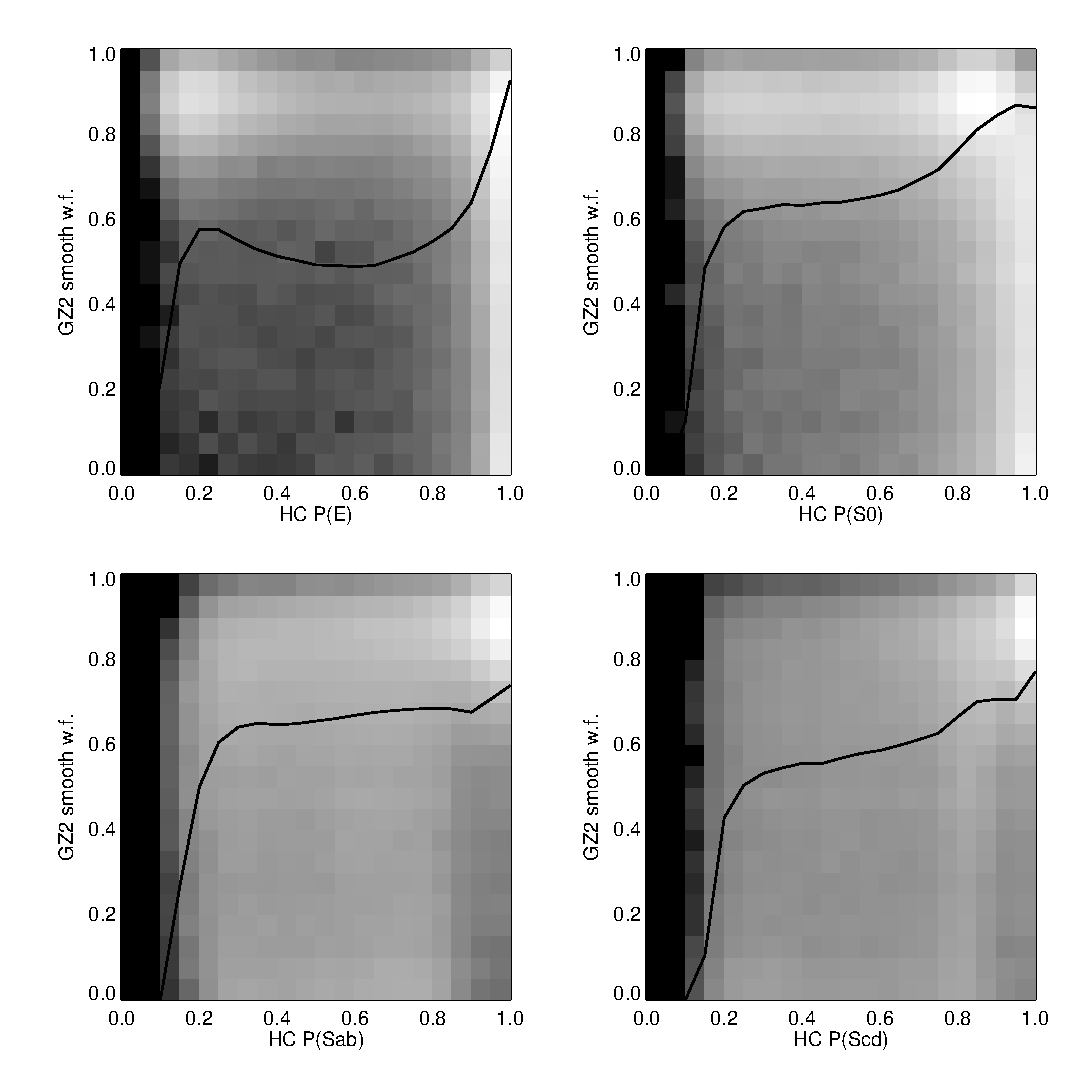
\includegraphics[angle=0,width=6.0in]{figures/hc_gz2_subclass.eps}
\caption{Left: GZ2 smooth weighted fraction as a function of \citet{hue11} early-type probability. Right: GZ2 features/disk weighted fraction as a function of HC late-type probability. Whiter values in both indicate a larger fraction of galaxies in that bin (logarithmic scale).
\label{fig-hc_gz2_subclass}}
\end{figure*}

\begin{figure}
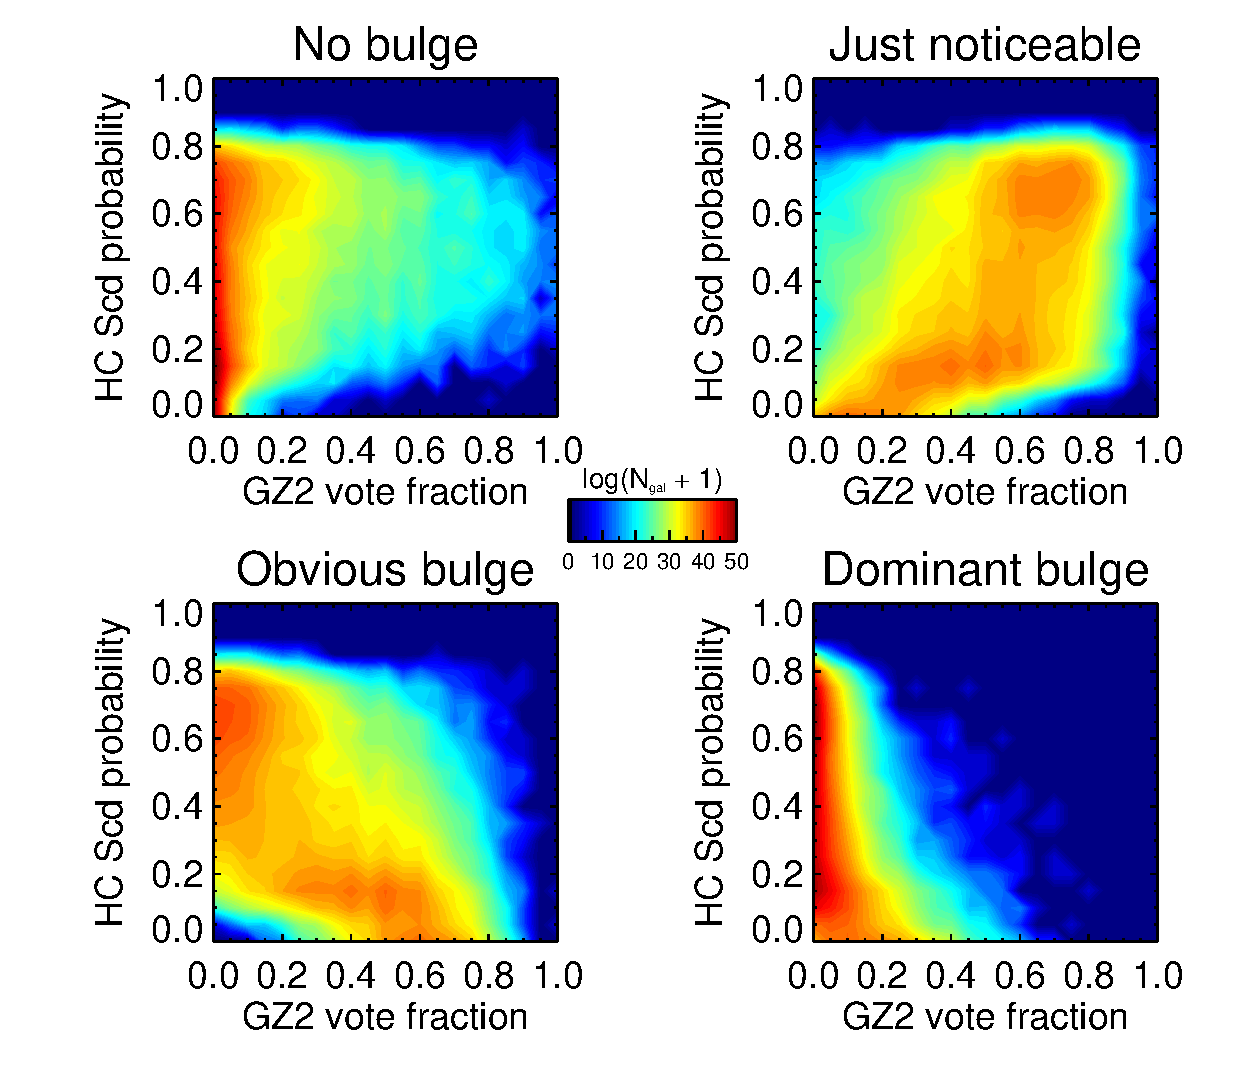
\includegraphics[angle=0,width=3.3in]{figures/hc_gz2_bulge_contour.eps}
\caption{\citet{hue11} early-type probability as a function of the GZ2 weighted vote fraction for bulge dominance. The colour of the contours is log~$(N_{gal} + 1)$, where $N_{gal}$ ranges from 0 to $1.5\times10^3$. Only galaxies with at least 10 classifications for Task~05 are shown.   
\label{fig-hc_gz2_bulge_contour}}
\end{figure}

\subsection{Other classification schemes}

Mention the volume classification of \citet{dev59}; recent developments by \citet{kor12,lau11,cap11,kra11} that have refined these ideas. \citet{but11} is a useful review of modern morphology. 

%%%%%%%%%%%%%%%%%%%%%%%%%%%%%%%%%%%%%%%
%%%%%%%%    Astronomy       %%%%%%%%%%%%%
%%%%%%%%%%%%%%%%%%%%%%%%%%%%%%%%%%%%%%%

%\section{Galaxy Wars}\label{sec_galaxywars}
\section{Astronomy}\label{sec_astronomy}

Statistical properties and demographics of galaxies to be placed here. At minimum, a table of the number of galaxies in each clean sample would be useful, plus a colour-magnitude diagram. Compare to early science results of EFIGI \citep{del11a} and NA10 \citep{nai10a,nai10b}

%%%%%%%%%%%%%%%%%%%%%%%%%%%%%%%%%%%%%%%
%%%%%%%%    Conclusions       %%%%%%%%%%%%%
%%%%%%%%%%%%%%%%%%%%%%%%%%%%%%%%%%%%%%%

\section{Conclusions}\label{sec_conclusions}

%%%%%%%%%%%%
%%% ACKNOWLEDGMENTS
%%%%%%%%%%%%

\section*{Acknowledgments}
The data in this paper are the result of the efforts of the Galaxy~Zoo~2 volunteers, without whom none of this work would have been possible. Their efforts are individually acknowledged at \url{http://authors.galaxyzoo.org}. 

Boilerplate for individual grants, Zooniverse support, etc.

This research made use of Montage, funded by the National Aeronautics and Space Administration's Earth Science Technology Office, Computation Technologies Project, under Cooperative Agreement Number NCC5-626 between NASA and the California Institute of Technology. Montage is maintained by the NASA/IPAC Infrared Science Archive.

Funding for the SDSS and SDSS-II has been provided by the Alfred P. Sloan Foundation, the Participating Institutions, the National Science Foundation, the U.S. Department of Energy, the National Aeronautics and Space Administration, the Japanese Monbukagakusho, the Max Planck Society, and the Higher Education Funding Council for England. The SDSS website is \url{http://www.sdss.org/}.

The SDSS is managed by the Astrophysical Research Consortium for the Participating Institutions. The Participating Institutions are the American Museum of Natural History, Astrophysical Institute Potsdam, University of Basel, University of Cambridge, Case Western Reserve University, University of Chicago, Drexel University, Fermilab, the Institute for Advanced Study, the Japan Participation Group, Johns Hopkins University, the Joint Institute for Nuclear Astrophysics, the Kavli Institute for Particle Astrophysics and Cosmology, the Korean Scientist Group, the Chinese Academy of Sciences (LAMOST), Los Alamos National Laboratory, the Max-Planck-Institute for Astronomy (MPIA), the Max-Planck-Institute for Astrophysics (MPA), New Mexico State University, Ohio State University, University of Pittsburgh, University of Portsmouth, Princeton University, the United States Naval Observatory, and the University of Washington.

%\clearpage

%%%%%%%%%%%%
%%% BIBLIOGRAPHY
%%%%%%%%%%%%

\bibliography{kwrefs}

\bsp

\newpage
\clearpage
\tabletypesize{\scriptsize}
\begin{deluxetable}{llcc|rrrrrr|rrrrrr|c}
\rotate
\tablecolumns{16}
\tablewidth{0pc}
\tablecaption{Morphological classifications of GZ2 main sample galaxies with spectra \label{tbl-mainclass}}
\tabletypesize{\scriptsize}
\tablehead{
 &  &  &  & 
\multicolumn{6}{c}{\underline{t01\_smooth\_or\_features\_a01\_smooth\_}} &
\multicolumn{6}{c}{\underline{t01\_smooth\_or\_features\_a02\_features\_or\_disk\_}} &
\colhead{$\dots$}
\\
\colhead{SDSS DR7 objID} & 
\colhead{sample} & 
\colhead{$N_{class}$} & 
\colhead{$N_{votes}$} & 
\colhead{count} & 
\colhead{wt\_count} & 
\colhead{fraction} & 
\colhead{wt\_fraction} & 
\colhead{debiased} &
\colhead{flag} &
\colhead{count} & 
\colhead{weight} & 
\colhead{fraction} & 
\colhead{wt\_fraction} & 
\colhead{debiased} &
\colhead{flag} &
\colhead{}
}
\small
\startdata
588017703996096547 & original &  44 & 349 &   1 &   0.1 & 0.023 & 0.002 & 0.002 & 0 &  42 &  42.0 & 0.955 & 0.975 & 0.975 & 1 \\
587738569780428805 & original &  45 & 185 &   5 &   5.0 & 0.111 & 0.115 & 0.115 & 0 &  38 &  38.0 & 0.844 & 0.873 & 0.873 & 1 \\
587735695913320507 & original &  46 & 372 &   0 &   0.0 & 0.000 & 0.000 & 0.000 & 0 &  44 &  44.0 & 0.957 & 0.966 & 0.966 & 1 \\
587742775634624545 & original &  45 & 289 &   8 &   8.0 & 0.178 & 0.178 & 0.178 & 0 &  37 &  37.0 & 0.822 & 0.822 & 0.822 & 1 \\
587732769983889439 &    extra &  49 & 210 &  12 &  12.0 & 0.245 & 0.249 & 0.249 & 0 &  36 &  36.0 & 0.735 & 0.748 & 0.748 & 0 \\
588017725475782665 &    extra &  42 & 149 &  27 &  27.0 & 0.643 & 0.686 & 0.686 & 0 &  12 &  12.0 & 0.286 & 0.305 & 0.305 & 0 \\
588017702391578633 & original &  45 & 356 &   0 &   0.0 & 0.000 & 0.000 & 0.000 & 0 &  45 &  45.0 & 1.000 & 1.000 & 1.000 & 1 \\
588297864730181658 & original &  45 & 206 &   4 &   4.0 & 0.089 & 0.091 & 0.091 & 0 &  39 &  38.5 & 0.867 & 0.871 & 0.871 & 1 \\
588017704545812500 & original &  43 & 360 &   0 &   0.0 & 0.000 & 0.000 & 0.000 & 0 &  43 &  43.0 & 1.000 & 1.000 & 1.000 & 1 \\
588017566564155399 &    extra &  43 & 244 &   6 &   6.0 & 0.140 & 0.143 & 0.143 & 0 &  35 &  35.0 & 0.814 & 0.833 & 0.833 & 1 \\
\enddata
\tablecomments{The full, machine-readable version of this table is available at http://data.galaxyzoo.org. A portion is shown here for guidance on form and content. The full table contains 252,750 rows (one for every galaxy in the sample), and 226 columns, with six variables for each of the 37 GZ2 morphology classifications. }
\end{deluxetable}

\tabletypesize{\scriptsize}
\begin{deluxetable}{llcc|rrrrrr|rrrrrr|c}
\rotate
\tablecolumns{16}
\tablewidth{0pc}
\tablecaption{Morphological classifications of GZ2 main sample galaxies with photo-$z$ \label{tbl-mainclass_photoz}}
\tabletypesize{\scriptsize}
\tablehead{
 &  &  &  & 
\multicolumn{6}{c}{\underline{t01\_smooth\_or\_features\_a01\_smooth\_}} &
\multicolumn{6}{c}{\underline{t01\_smooth\_or\_features\_a02\_features\_or\_disk\_}} &
\colhead{$\dots$}
\\
\colhead{SDSS DR7 objid} & 
\colhead{sample} & 
\colhead{$N_{class}$} & 
\colhead{$N_{votes}$} & 
\colhead{count} & 
\colhead{wt\_count} & 
\colhead{fraction} & 
\colhead{wt\_fraction} & 
\colhead{debiased} &
\colhead{flag} &
\colhead{count} & 
\colhead{weight} & 
\colhead{fraction} & 
\colhead{wt\_fraction} & 
\colhead{debiased} &
\colhead{flag} &
\colhead{}
}
\small
\startdata
587722981736579107 & original &  43 & 181 &  27 &  27.0 & 0.628 & 0.648 & 0.648 & 0 &  14 &  14.0 & 0.326 & 0.336 & 0.336 & 0 \\
587722981741691055 & original &  44 & 133 &  40 &  40.0 & 0.909 & 0.909 & 0.909 & 1 &   1 &   1.0 & 0.023 & 0.023 & 0.023 & 0 \\
587722981745819655 & original &  46 & 221 &  17 &  17.0 & 0.370 & 0.378 & 0.378 & 0 &  22 &  22.0 & 0.478 & 0.489 & 0.489 & 0 \\
587722981746082020 & original &  44 & 172 &  31 &  31.0 & 0.705 & 0.771 & 0.386 & 0 &   6 &   6.0 & 0.136 & 0.149 & 0.814 & 1 \\
587722981746344092 & original &  43 & 358 &   0 &   0.0 & 0.000 & 0.000 & 0.000 & 0 &  43 &  43.0 & 1.000 & 1.000 & 1.000 & 1 \\
587722981747982511 & original &  45 & 156 &  37 &  37.0 & 0.822 & 0.850 & 0.578 & 0 &   3 &   3.0 & 0.067 & 0.069 & 0.289 & 0 \\
587722981748375814 & original &  52 & 198 &  44 &  44.0 & 0.846 & 0.846 & 0.674 & 0 &   8 &   8.0 & 0.154 & 0.154 & 0.204 & 0 \\
587722981748768914 & original &  46 & 350 &   3 &   3.0 & 0.065 & 0.065 & 0.117 & 0 &  43 &  43.0 & 0.935 & 0.935 & 0.935 & 1 \\
587722981748768984 & original &  42 & 140 &  37 &  36.2 & 0.881 & 0.900 & 0.699 & 0 &   4 &   4.0 & 0.095 & 0.100 & 0.128 & 0 \\
587722981749031027 & original &  50 & 158 &  46 &  45.8 & 0.920 & 0.932 & 0.710 & 0 &   2 &   1.4 & 0.040 & 0.028 & 0.107 & 0 \\
\enddata
\tablecomments{The full, machine-readable version of this table is available at http://data.galaxyzoo.org. A portion is shown here for guidance on form and content, which are identical to those in Table~\ref{tbl-mainclass}.}
\end{deluxetable}

\newpage
\clearpage
\tabletypesize{\scriptsize}
\begin{deluxetable}{lcc|rrrrrr|rrrrrr|c}
\rotate
\tablecolumns{16}
\tablewidth{0pc}
\tablecaption{Morphological classifications of GZ2 Stripe~82 coadded galaxies with spectra \label{tbl-stripe82}}
\tabletypesize{\scriptsize}
\tablehead{
 &  &   & 
\multicolumn{6}{c}{\underline{t01\_smooth\_or\_features\_a01\_smooth\_}} &
\multicolumn{6}{c}{\underline{t01\_smooth\_or\_features\_a02\_features\_or\_disk\_}} &
\colhead{$\dots$}
\\
\colhead{Stripe82 objID} & 
\colhead{$N_{class}$} & 
\colhead{$N_{votes}$} & 
\colhead{count} & 
\colhead{wt\_count} & 
\colhead{fraction} & 
\colhead{wt\_fraction} & 
\colhead{debiased} &
\colhead{flag} &
\colhead{count} & 
\colhead{weight} & 
\colhead{fraction} & 
\colhead{wt\_fraction} & 
\colhead{debiased} &
\colhead{flag} &
\colhead{}
}
\small
\startdata
8647474690312307154 &   16 &  72 &  10 &  10.0 & 0.625 & 0.625 & 0.218 & 0 &   5 &   5.0 & 0.312 & 0.312 & 0.775 & 0 \\
8647474690312307877 &   21 &  84 &  17 &  17.0 & 0.810 & 0.810 & 0.810 & 1 &   4 &   4.0 & 0.190 & 0.190 & 0.190 & 0 \\
8647474690312308318 &   23 &  88 &  18 &  18.0 & 0.783 & 0.783 & 0.783 & 0 &   4 &   4.0 & 0.174 & 0.174 & 0.174 & 0 \\
8647474690312308880 &   16 &  48 &  16 &  16.0 & 1.000 & 1.000 & 1.000 & 1 &   0 &   0.0 & 0.000 & 0.000 & 0.000 & 0 \\
8647474690312373464 &   23 &  89 &  17 &  17.0 & 0.739 & 0.739 & 0.739 & 0 &   4 &   4.0 & 0.174 & 0.174 & 0.174 & 0 \\
8647474690312438284 &   11 &  91 &   0 &   0.0 & 0.000 & 0.000 & 0.000 & 0 &  11 &  11.0 & 1.000 & 1.000 & 1.000 & 1 \\
8647474690312505086 &   12 &  65 &   4 &   3.4 & 0.333 & 0.295 & 0.295 & 0 &   8 &   8.0 & 0.667 & 0.705 & 0.705 & 0 \\
8647474690312832559 &   23 &  75 &  14 &  14.0 & 0.609 & 0.629 & 0.280 & 0 &   4 &   4.0 & 0.174 & 0.180 & 0.826 & 1 \\
8647474690312898532 &   26 & 129 &  12 &  12.0 & 0.462 & 0.462 & 0.462 & 0 &  14 &  14.0 & 0.538 & 0.538 & 0.538 & 0 \\
8647474690312962734 &   20 &  69 &  18 &  17.0 & 0.900 & 0.895 & 0.895 & 1 &   2 &   2.0 & 0.100 & 0.105 & 0.105 & 0 \\
\enddata
\tablecomments{The full, machine-readable version of this table is available at http://data.galaxyzoo.org. A portion is shown here for guidance on form and content, which are identical to those in Table~\ref{tbl-mainclass}. Classifications here are for the coadded images (version~2) from Stripe~82, which goes to a deeper magnitude limit and has a better angular resolution than galaxies in the main sample.}
\end{deluxetable}

\newpage
\clearpage
\tabletypesize{\scriptsize}
\begin{deluxetable}{lccrrrr}
\tablecolumns{16}
\tablewidth{0pc}
\tablecaption{GZ2 weighted vote fractions for the main and Stripe~82 normal-depth samples \label{tbl-stripe82compare}}
\tabletypesize{\scriptsize}
\tablehead{
 & \multicolumn{2}{c}{\underline{Mean weighted vote fraction}} & \multicolumn{2}{c}{\underline{Number of galaxies}} & \multicolumn{2}{c}{\underline{Sample comparison}} \\
\colhead{User task and answer} & 
\colhead{Main} & 
\colhead{Stripe~82} & 
\colhead{Main} & 
\colhead{Stripe~82} &
\colhead{$f_m - f_s$} & 
\colhead{$f_m/f_s$} 
}
\small
\startdata
T01\_SMOOTH\_OR\_FEATURES\_A01\_SMOOTH                      &      0.642 &      0.613 &     273783 &       8437 &       0.029 &       1.048 \\
T01\_SMOOTH\_OR\_FEATURES\_A02\_FEATURES\_OR\_DISK          &      0.325 &      0.352 &     273783 &       8437 &      -0.027 &       0.924 \\
T01\_SMOOTH\_OR\_FEATURES\_A03\_STAR\_OR\_ARTIFACT          &      0.033 &      0.036 &     273783 &       8437 &      -0.003 &       0.924 \\
T02\_EDGEON\_A04\_YES                                       &      0.234 &      0.229 &     118147 &       4110 &       0.005 &       1.020 \\
T02\_EDGEON\_A05\_NO                                        &      0.766 &      0.771 &     118147 &       4110 &      -0.005 &       0.994 \\
T03\_BAR\_A06\_BAR                                          &      0.287 &      0.292 &      87647 &       3077 &      -0.004 &       0.986 \\
T03\_BAR\_A07\_NO\_BAR                                      &      0.713 &      0.708 &      87647 &       3077 &       0.004 &       1.006 \\
T04\_SPIRAL\_A08\_SPIRAL                                    &      0.660 &      0.674 &      87621 &       3077 &      -0.014 &       0.980 \\
T04\_SPIRAL\_A09\_NO\_SPIRAL                                &      0.340 &      0.326 &      87621 &       3077 &       0.014 &       1.042 \\
T05\_BULGE\_PROMINENCE\_A10\_NO\_BULGE                      &      0.129 &      0.114 &      87608 &       3076 &       0.015 &       1.129 \\
T05\_BULGE\_PROMINENCE\_A11\_JUST\_NOTICEABLE               &      0.479 &      0.491 &      87608 &       3076 &      -0.012 &       0.976 \\
T05\_BULGE\_PROMINENCE\_A12\_OBVIOUS                        &      0.321 &      0.333 &      87608 &       3076 &      -0.011 &       0.966 \\
T05\_BULGE\_PROMINENCE\_A13\_DOMINANT                       &      0.070 &      0.062 &      87608 &       3076 &       0.008 &       1.134 \\
T06\_ODD\_A14\_YES                                          &      0.199 &      0.185 &     273636 &       8391 &       0.014 &       1.073 \\
T06\_ODD\_A15\_NO                                           &      0.801 &      0.815 &     273636 &       8391 &      -0.014 &       0.983 \\
T07\_ROUNDED\_A16\_COMPLETELY\_ROUND                        &      0.330 &      0.326 &     229974 &       6956 &       0.005 &       1.014 \\
T07\_ROUNDED\_A17\_IN\_BETWEEN                              &      0.496 &      0.501 &     229974 &       6956 &      -0.004 &       0.991 \\
T07\_ROUNDED\_A18\_CIGAR\_SHAPED                            &      0.173 &      0.174 &     229974 &       6956 &      -0.000 &       0.999 \\
T08\_ODD\_FEATURE\_A19\_RING                                &      0.147 &      0.178 &      72439 &       2114 &      -0.031 &       0.827 \\
T08\_ODD\_FEATURE\_A20\_LENS\_OR\_ARC                       &      0.045 &      0.040 &      72439 &       2114 &       0.005 &       1.122 \\
T08\_ODD\_FEATURE\_A21\_DISTURBED                           &      0.121 &      0.125 &      72439 &       2114 &      -0.003 &       0.973 \\
T08\_ODD\_FEATURE\_A22\_IRREGULAR                           &      0.177 &      0.170 &      72439 &       2114 &       0.007 &       1.039 \\
T08\_ODD\_FEATURE\_A23\_OTHER                               &      0.282 &      0.245 &      72439 &       2114 &       0.037 &       1.152 \\
T08\_ODD\_FEATURE\_A24\_MERGER                              &      0.212 &      0.209 &      72439 &       2114 &       0.003 &       1.015 \\
T08\_ODD\_FEATURE\_A38\_DUST\_LANE                          &      0.016 &      0.034 &      72439 &       2114 &      -0.018 &       0.475 \\
T09\_BULGE\_SHAPE\_A25\_ROUNDED                             &      0.538 &      0.567 &      21496 &        746 &      -0.029 &       0.948 \\
T09\_BULGE\_SHAPE\_A26\_BOXY                                &      0.103 &      0.096 &      21496 &        746 &       0.007 &       1.077 \\
T09\_BULGE\_SHAPE\_A27\_NO\_BULGE                           &      0.359 &      0.338 &      21496 &        746 &       0.022 &       1.065 \\
T10\_ARMS\_WINDING\_A28\_TIGHT                              &      0.370 &      0.392 &      55800 &       2052 &      -0.022 &       0.943 \\
T10\_ARMS\_WINDING\_A29\_MEDIUM                             &      0.417 &      0.405 &      55800 &       2052 &       0.011 &       1.028 \\
T10\_ARMS\_WINDING\_A30\_LOOSE                              &      0.214 &      0.203 &      55800 &       2052 &       0.011 &       1.054 \\
T11\_ARMS\_NUMBER\_A31\_1                                   &      0.074 &      0.067 &      55805 &       2053 &       0.008 &       1.117 \\
T11\_ARMS\_NUMBER\_A32\_2                                   &      0.501 &      0.478 &      55805 &       2053 &       0.023 &       1.048 \\
T11\_ARMS\_NUMBER\_A33\_3                                   &      0.093 &      0.098 &      55805 &       2053 &      -0.005 &       0.950 \\
T11\_ARMS\_NUMBER\_A34\_4                                   &      0.038 &      0.043 &      55805 &       2053 &      -0.005 &       0.884 \\
T11\_ARMS\_NUMBER\_A36\_MORE\_THAN\_4                       &      0.030 &      0.033 &      55805 &       2053 &      -0.002 &       0.934 \\
T11\_ARMS\_NUMBER\_A37\_CANT\_TELL                          &      0.263 &      0.281 &      55805 &       2053 &      -0.019 &       0.934 \\
\enddata
\tablecomments{Data for each task is only for galaxies with at least 10 total responses to the classification question.}
\end{deluxetable}

\label{lastpage}

\end{document}
